\documentclass[12pt,a4paper]{article}
% Course report - Topic 13: Multi-Delivery Robot. Compile with pdfLaTeX (Overleaf default).
\usepackage[T1]{fontenc}
\usepackage[utf8]{inputenc}
\IfFileExists{newtxtext.sty}{\usepackage{newtxtext,newtxmath}}{\usepackage{mathptmx}}
\usepackage[a4paper,top=2.5cm,bottom=2.5cm,left=3cm,right=2cm]{geometry}
\usepackage{amsmath,amssymb}
\usepackage{graphicx}
\usepackage{longtable,booktabs,array,calc}
\usepackage{etoolbox}
\usepackage{listings}
\usepackage{xcolor}
\usepackage{tikz}
\usepackage{float}
\usepackage[font=small,labelfont=bf]{caption}
\usepackage{fancyhdr}
\usepackage{newunicodechar}
\usepackage[hidelinks]{hyperref}

\linespread{1.2}
\setlength{\parskip}{4pt}
\setlength{\parindent}{0pt}
\providecommand{\tightlist}{\setlength{\itemsep}{0pt}\setlength{\parskip}{0pt}}
\providecommand{\real}[1]{#1}
\AtBeginEnvironment{longtable}{\small\setlength{\tabcolsep}{4pt}}
\setlength{\LTpre}{6pt}\setlength{\LTpost}{6pt}

\definecolor{pkblue}{HTML}{233871}
\definecolor{pkorange}{HTML}{F26B21}
\definecolor{codebg}{HTML}{F4F5F8}
\lstset{basicstyle=\ttfamily\scriptsize,backgroundcolor=\color{codebg},frame=single,rulecolor=\color{codebg},
  columns=fixed,keepspaces=true,breaklines=true,xleftmargin=4pt,xrightmargin=4pt,aboveskip=6pt,belowskip=6pt}

% Unicode characters used in the text
\newunicodechar{±}{\ensuremath{\pm}}
\newunicodechar{·}{\ensuremath{\cdot}}
\newunicodechar{×}{\ensuremath{\times}}
\newunicodechar{α}{\ensuremath{\alpha}}
\newunicodechar{γ}{\ensuremath{\gamma}}
\newunicodechar{ε}{\ensuremath{\varepsilon}}
\newunicodechar{λ}{\ensuremath{\lambda}}
\newunicodechar{σ}{\ensuremath{\sigma}}
\newunicodechar{τ}{\ensuremath{\tau}}
\newunicodechar{ᵢ}{\ensuremath{_i}}
\newunicodechar{′}{\ensuremath{'}}
\newunicodechar{⁵}{\textsuperscript{5}}
\newunicodechar{⁻}{\textsuperscript{\textminus}}
\newunicodechar{₀}{\textsubscript{0}}
\newunicodechar{₁}{\textsubscript{1}}
\newunicodechar{₂}{\textsubscript{2}}
\newunicodechar{₃}{\textsubscript{3}}
\newunicodechar{→}{\ensuremath{\rightarrow}}
\newunicodechar{−}{\ensuremath{-}}
\newunicodechar{…}{\ldots}

\pagestyle{fancy}
\fancyhf{}
\fancyfoot[R]{\thepage}
\fancyfoot[L]{\small\color{gray}Topic 13 -- Multi-Delivery Robot}
\renewcommand{\headrulewidth}{0pt}

\begin{document}

% ======================= COVER =======================
\begin{titlepage}
\begin{tikzpicture}[remember picture,overlay]
  \draw[line width=1.2pt] ([xshift=1.5cm,yshift=-1.5cm]current page.north west) rectangle ([xshift=-1.5cm,yshift=1.5cm]current page.south east);
  \draw[line width=0.6pt] ([xshift=-2.3cm,yshift=-2.1cm]current page.north east) rectangle ++(-1.5cm,-1.0cm);
\end{tikzpicture}
\centering
\vspace*{0.1cm}
{\large\bfseries PHENIKAA UNIVERSITY\par}
{\large\bfseries SCHOOL OF ENGINEERING AND TECHNOLOGY\par}
{\large\bfseries\underline{FACULTY OF ELECTRICAL AND ELECTRONIC ENGINEERING}\par}
\vspace{0.5cm}

\includegraphics[width=3.2cm]{figures/phenikaa_logo.png}\par
\vspace{0.5cm}
{\large\bfseries COURSE PROJECT REPORT\par}
{\large\bfseries REINFORCEMENT LEARNING\par}
\vspace{0.5cm}
{\bfseries Title of the project:\par}
{\bfseries Topic 13 -- Multi-Delivery Robot:\par
Tabular Q-learning, SARSA and Monte Carlo ES\par
on Four Maps of Increasing Difficulty\par}
\vspace{0.5cm}
{\small
\begin{tabular}{@{}l l l l@{}}
\textbf{Student:} & Nguyen Quang Trung & \textbf{Student ID:} & 22011211\\[2pt]
\textbf{Supervisor:} & MSc. Vu Hoang Dieu & \textbf{Major:} & Electrical and Electronic Engineering\\
\end{tabular}\par}
\vspace{0.6cm}
\setlength{\fboxsep}{0pt}
\fbox{\begin{minipage}[t][2.6cm]{4.2cm}\centering\vspace{4pt}{\small Score}\end{minipage}}\par
\vspace{0.6cm}
{\renewcommand{\arraystretch}{1.4}
\begin{tabular}{|p{6.3cm}|p{6.3cm}|}
\hline
\centering Lecturer 1 & \centering Lecturer 2 \tabularnewline
\hline
\parbox[b][2.4cm][b]{6.3cm}{\centering MSc. Vu Hoang Dieu\\[4pt]} & \\
\hline
\end{tabular}\par}
\vfill
{Hanoi, November 2026\par}
\vspace*{0.2cm}
\end{titlepage}

% ======================= FRONT MATTER =======================
\pagenumbering{roman}
{\linespread{1.0}\selectfont
\tableofcontents
\clearpage
\listoffigures
\listoftables
\clearpage}
\pagenumbering{arabic}

\hypertarget{problem-statement}{%
\section{Problem statement}\label{problem-statement}}

A robot moves on a grid of square cells, picks up several parcels at
their pickup cells (P) and delivers them to their drop cells (D); the
agent learns by itself the pickup and delivery order that maximises the
total reward. The environment is a custom gymnasium.Env that follows the
logic of Taxi-v3. The agent learns a Q table with three algorithms:
Q-learning, SARSA and Monte Carlo ES; no DQN or function approximation
is used.

There are 4 maps of increasing difficulty, and each level adds one new
mechanic: more parcels, capacity 1, a deadline, a booster cell. After
improving exploration and increasing the number of episodes, all three
algorithms find the optimal route from every start cell on all 4 maps,
in 5/5 seeds. Section 10 then puts the robot in every reachable state,
not only at a start cell, to find where each algorithm still goes wrong.
The training loops are compiled with numba, so millions of episodes run
in a few tens of seconds.

\begin{longtable}[]{@{}
  >{\raggedright\arraybackslash}p{(\columnwidth - 2\tabcolsep) * \real{0.3000}}
  >{\raggedright\arraybackslash}p{(\columnwidth - 2\tabcolsep) * \real{0.7000}}@{}}
\caption{Source code structure}\label{tab:1}\\
\toprule\noalign{}
\begin{minipage}[b]{\linewidth}\raggedright
\textbf{File / folder}
\end{minipage} & \begin{minipage}[b]{\linewidth}\raggedright
\textbf{Role}
\end{minipage} \\
\midrule\noalign{}
\endfirsthead
\caption[]{(continued)}\\
\toprule\noalign{}
\begin{minipage}[b]{\linewidth}\raggedright
\textbf{File / folder}
\end{minipage} & \begin{minipage}[b]{\linewidth}\raggedright
\textbf{Role}
\end{minipage} \\
\midrule\noalign{}
\endhead
\bottomrule\noalign{}
\endlastfoot
configs/*.json & The 4 maps by level (grid, parcels, capacity, deadline,
booster cell, rewards, number of episodes) \\
delivery\_env.py & MultiDeliveryEnv environment: state encoding,
transition function, rewards; precomputed transition tables NS, R, D \\
agents.py & Q-learning, SARSA and Monte Carlo ES (compiled with numba),
ε-greedy, greedy policy rollout \\
planner.py & Value Iteration for the optimal return and Q* as a
reference \\
experiments.py & Runs every experiment (5 seeds); saves to results/ \\
convergence.py & Measures how the Q table converges to Q* \\
failure\_cases.py & Puts the robot in every reachable state and finds
where the greedy policy goes wrong (loops, late deliveries, illegal
actions, longer routes); draws Figure 11 \\
plots.py & Draws the maps, accuracy, learning curves, policies, value
heatmaps and reward experiments \\
demo.py & Runs one episode with the learned policy and prints every
step \\
play.py & Play the game yourself with the keyboard: W/A/S/D move, J
picks up, K drops \\
colab\_train.ipynb & Runs every experiment on Google Colab \\
README.md & Explains every file, the formulas and how to run them \\
\end{longtable}

\hypertarget{mdp-formulation}{%
\section{MDP formulation}\label{mdp-formulation}}

At each step the robot is in state s, takes action a, receives reward r
and moves to state s′; the environment is deterministic, so (s, a)
always leads to exactly one s′.

\hypertarget{state}{%
\subsection{State}\label{state}}

A state is a tuple with 5 components:

\[s = \left( \text{row, col},\sigma_{1},\ldots,\sigma_{N},\tau,b \right)\]

\[\sigma_{i} \in \{ 0,\text{ }1,\text{ }2\},\text{     }\tau \in \{ 0,\ldots,T_{d}\},\text{     }b \in \{ 0,\text{ }1,\text{ }2\}\]

\begin{itemize}
\item
  σᵢ is the status of parcel i: 0 = waiting, 1 = being carried, 2 =
  delivered.
\item
  τ is the deadline clock (S3 and S4 only), and b is the booster status
  (S4 only): 0 = unused, 1 = active, 2 = used up.
\end{itemize}

\hypertarget{actions-and-rewards}{%
\subsection{Actions and rewards}\label{actions-and-rewards}}

There are 6 actions: Up, Down, Left, Right, Pickup, Drop.

\begin{longtable}[]{@{}
  >{\raggedright\arraybackslash}p{(\columnwidth - 2\tabcolsep) * \real{0.7000}}
  >{\raggedright\arraybackslash}p{(\columnwidth - 2\tabcolsep) * \real{0.3000}}@{}}
\caption{Default rewards}\label{tab:2}\\
\toprule\noalign{}
\begin{minipage}[b]{\linewidth}\raggedright
\textbf{Event}
\end{minipage} & \begin{minipage}[b]{\linewidth}\raggedright
\textbf{Reward}
\end{minipage} \\
\midrule\noalign{}
\endfirsthead
\caption[]{(continued)}\\
\toprule\noalign{}
\begin{minipage}[b]{\linewidth}\raggedright
\textbf{Event}
\end{minipage} & \begin{minipage}[b]{\linewidth}\raggedright
\textbf{Reward}
\end{minipage} \\
\midrule\noalign{}
\endhead
\bottomrule\noalign{}
\endlastfoot
Each step (including bumping into a wall) & −1 \\
Correct delivery of one parcel (per-order reward) & +20 \\
Pickup/Drop in the wrong cell or over capacity & −10 (plus the step
penalty) \\
Deadline parcel not delivered when τ reaches T\textsubscript{d} (once) &
−30 \\
\end{longtable}

\hypertarget{transition-function}{%
\subsection{Transition function}\label{transition-function}}

\begin{enumerate}
\def\labelenumi{\arabic{enumi}.}
\item
  \textbf{Move:} if the new cell is inside the grid and not a wall, the
  robot moves there; otherwise it stays in place. Entering the booster
  cell when b = 0 sets b = 1.
\item
  \textbf{Pickup:} if a parcel i is waiting in the current cell and the
  robot carries fewer parcels than its capacity (2 if b = 1, otherwise
  capacity), then σᵢ: 0 → 1.
\item
  \textbf{Drop:} if the robot carries parcel i and the current cell is
  its drop cell, then σᵢ: 1 → 2 and the order\textquotesingle s reward
  is paid. If b = 1 and the robot has just become empty-handed, b = 2
  (the booster trip is over).
\item
  \textbf{Clock:} if the deadline parcel has been delivered, τ =
  T\textsubscript{d}; otherwise τ increases by 1 (capped at
  T\textsubscript{d}), and the late penalty is applied at the moment τ
  reaches T\textsubscript{d}.
\end{enumerate}

\hypertarget{termination}{%
\subsection{Termination}\label{termination}}

An episode is \textbf{terminated} when every σᵢ = 2 and
\textbf{truncated} when max\_steps runs out (100 / 150 / 200 / 300 for
S1--S4). Truncation is a time limit, not a terminal state, so Q-learning
and SARSA still bootstrap on the last step.

\hypertarget{extra-variables-for-the-markov-property}{%
\subsection{Extra variables for the Markov
property}\label{extra-variables-for-the-markov-property}}

\begin{itemize}
\item
  \textbf{τ:} the late penalty depends on how many steps have passed, so
  without τ two visits to the same cell with the same parcel statuses
  could have different futures. Once the deadline parcel is delivered, τ
  is merged into T\textsubscript{d} because time no longer affects the
  reward.
\item
  \textbf{b:} the capacity depends on whether the robot has passed the
  booster cell and whether that trip is over; the position and σ alone
  cannot tell.
\item
  \textbf{σ = 1 (carrying)} replaces a separate "current load" variable:
  the number of parcels carried is the number of σᵢ equal to 1.
\end{itemize}

\hypertarget{state-encoding-and-state-space-size}{%
\section{State encoding and state-space
size}\label{state-encoding-and-state-space-size}}

The statuses of the N parcels are read as an N-digit base-3 number, and
the whole tuple is then packed into a single integer that is the row
index of the Q table (encode / decode in delivery\_env.py).

\[\text{code} = \sum_{i = 1}^{N}{\sigma_{i} \cdot 3^{i - 1}} \in \{ 0,\ldots,3^{N} - 1\}\]

\[\text{idx} = \left( \left( \left( \text{row} \cdot W + \text{col} \right) \cdot 3^{N} + \text{code} \right) \cdot T + \tau \right) \cdot B + b\]

The size of the encoded state space is the product of the number of
values of each component:

\[|S| = H \cdot W \cdot 3^{N} \cdot T \cdot B\]

\[T = \left\{ \begin{aligned}
 & T_{d} + 1,\text{ if there is a deadline parcel} \\
 & 1,\text{ otherwise}
\end{aligned} \right.\ \]

\[B = \left\{ \begin{aligned}
 & 3,\text{ if the map has a booster cell} \\
 & 1,\text{ otherwise}
\end{aligned} \right.\ \]

For S3 and S4:

\[\begin{aligned}
{|S|}_{\text{S3}} & = 7 \cdot 7 \cdot 3^{3} \cdot 21 \cdot 1 = \text{27,783} \\
{|S|}_{\text{S4}} & = 8 \cdot 8 \cdot 3^{4} \cdot 23 \cdot 3 = \text{357,696}
\end{aligned}\]

\textbf{Example on S3} (7x7 grid, N = 3, T = 21, B = 1): the robot is in
row 2, column 3, A has been delivered (σ₁ = 2), B is being carried (σ₂ =
1), C is waiting (σ₃ = 0), τ = 7:

\[\begin{aligned}
\text{code} & = 2 \cdot 3^{0} + 1 \cdot 3^{1} + 0 \cdot 3^{2} = 5 \\
\text{idx} & = (((2 \cdot 7 + 3) \cdot 27 + 5) \cdot 21 + 7) \cdot 1 + 0 \\
 & = (17 \cdot 27 + 5) \cdot 21 + 7 = 464 \cdot 21 + 7 = 9751
\end{aligned}\]

decode reverses this with successive divmod operations, splitting off
one component from the right each time:

\[\begin{aligned}
9751 & = 464 \cdot 21 + 7 \Rightarrow \tau = 7 \\
464 & = 17 \cdot 27 + 5 \Rightarrow \text{code} = 5 \Rightarrow \left( \sigma_{1},\sigma_{2},\sigma_{3} \right) = \left( 2,\text{ }1,\text{ }0 \right) \\
17 & = 2 \cdot 7 + 3 \Rightarrow \text{row} = 2,\text{ col} = 3
\end{aligned}\]

In the code these are the two methods encode() and decode() of
MultiDeliveryEnv in delivery\_env.py (comments translated). The integer
that encode() returns is the \textbf{state code} of the state: it is the
row of the Q table and of the transition tables NS, R and D, and Section
10 and Appendix A use it to point at the exact states where the robot
goes wrong.

\begin{lstlisting}
def encode(self, state):             # delivery_env.py, MultiDeliveryEnv
    r, c, status, tau, boost = state
    code = 0
    for i, s in enumerate(status):   # parcel statuses = base-3 digits
        code += s * 3 ** i
    idx = r * self.W + c             # cell
    idx = idx * self.n_codes + code  # n_codes = 3^N
    idx = idx * self.n_tau + tau     # n_tau = T_d + 1 (1 if no deadline)
    idx = idx * self.n_boost + boost # n_boost = 3 (1 if no booster)
    return idx                       # state code = row of Q, NS, R, D
\end{lstlisting}

\begin{lstlisting}
def decode(self, idx):               # the reverse: one divmod per part
    idx, boost = divmod(idx, self.n_boost)
    idx, tau = divmod(idx, self.n_tau)
    pos, code = divmod(idx, self.n_codes)
    r, c = divmod(pos, self.W)
    status = []
    for _ in range(self.N):
        code, s = divmod(code, 3)
        status.append(s)
    return (r, c, tuple(status), tau, boost)
\end{lstlisting}

\begin{longtable}[]{@{}
  >{\raggedright\arraybackslash}p{(\columnwidth - 16\tabcolsep) * \real{0.2597}}
  >{\raggedright\arraybackslash}p{(\columnwidth - 16\tabcolsep) * \real{0.0854}}
  >{\raggedright\arraybackslash}p{(\columnwidth - 16\tabcolsep) * \real{0.0976}}
  >{\raggedright\arraybackslash}p{(\columnwidth - 16\tabcolsep) * \real{0.1367}}
  >{\raggedright\arraybackslash}p{(\columnwidth - 16\tabcolsep) * \real{0.0594}}
  >{\raggedright\arraybackslash}p{(\columnwidth - 16\tabcolsep) * \real{0.0585}}
  >{\raggedright\arraybackslash}p{(\columnwidth - 16\tabcolsep) * \real{0.1207}}
  >{\raggedright\arraybackslash}p{(\columnwidth - 16\tabcolsep) * \real{0.1299}}
  >{\raggedright\arraybackslash}p{(\columnwidth - 16\tabcolsep) * \real{0.0520}}@{}}
\caption{State-space and action-space size}\label{tab:3}\\
\toprule\noalign{}
\begin{minipage}[b]{\linewidth}\raggedright
\textbf{Setting}
\end{minipage} & \begin{minipage}[b]{\linewidth}\raggedright
\textbf{Grid}
\end{minipage} & \begin{minipage}[b]{\linewidth}\raggedright
\textbf{Parcels}
\end{minipage} & \begin{minipage}[b]{\linewidth}\raggedright
\textbf{Capacity}
\end{minipage} & \begin{minipage}[b]{\linewidth}\raggedright
\textbf{T}
\end{minipage} & \begin{minipage}[b]{\linewidth}\raggedright
\textbf{B}
\end{minipage} & \begin{minipage}[b]{\linewidth}\raggedright
\textbf{Encoded $|S|$}
\end{minipage} & \begin{minipage}[b]{\linewidth}\raggedright
\textbf{Reachable (BFS)}
\end{minipage} & \begin{minipage}[b]{\linewidth}\raggedright
\textbf{\textbar A\textbar{}}
\end{minipage} \\
\midrule\noalign{}
\endfirsthead
\caption[]{(continued)}\\
\toprule\noalign{}
\begin{minipage}[b]{\linewidth}\raggedright
\textbf{Setting}
\end{minipage} & \begin{minipage}[b]{\linewidth}\raggedright
\textbf{Grid}
\end{minipage} & \begin{minipage}[b]{\linewidth}\raggedright
\textbf{Parcels}
\end{minipage} & \begin{minipage}[b]{\linewidth}\raggedright
\textbf{Capacity}
\end{minipage} & \begin{minipage}[b]{\linewidth}\raggedright
\textbf{T}
\end{minipage} & \begin{minipage}[b]{\linewidth}\raggedright
\textbf{B}
\end{minipage} & \begin{minipage}[b]{\linewidth}\raggedright
\textbf{Encoded $|S|$}
\end{minipage} & \begin{minipage}[b]{\linewidth}\raggedright
\textbf{Reachable (BFS)}
\end{minipage} & \begin{minipage}[b]{\linewidth}\raggedright
\textbf{\textbar A\textbar{}}
\end{minipage} \\
\midrule\noalign{}
\endhead
\bottomrule\noalign{}
\endlastfoot
S1 -- level 1 & 5x5 & 2 & 2 & 1 & 1 & 225 & 186 & 6 \\
S2 -- level 2 & 6x6 & 3 & 1 & 1 & 1 & 972 & 535 & 6 \\
S3 -- level 3 & 7x7 & 3 & 1 & 21 & 1 & 27,783 & 4,027 & 6 \\
S4 -- level 4 & 8x8 & 4 & 1 (2 with booster) & 23 & 3 & 357,696 & 15,612
& 6 \\
\end{longtable}

\begin{figure}[htbp]
\centering
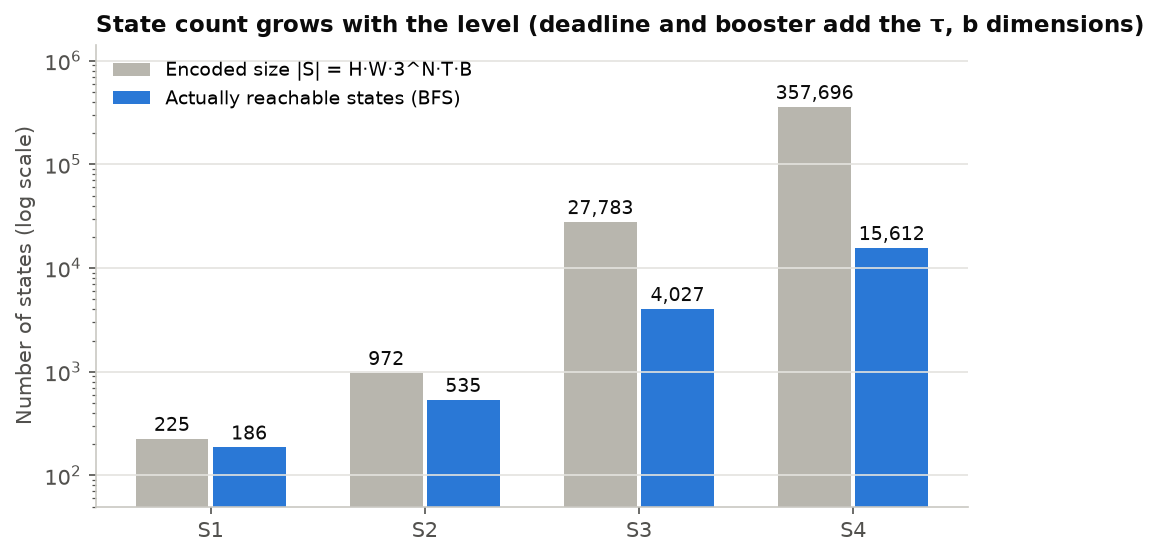
\includegraphics[width=0.80\linewidth,height=0.62\textheight,keepaspectratio]{figures/fig01.png}
\caption{Encoded size and number of actually reachable states of the four maps (log scale)}\label{fig:1}
\end{figure}

The number of reachable states is far below $|S|$ because
walls can never be occupied, capacity 1 removes the combinations with
two σᵢ = 1 (20/27 combinations remain with 3 parcels, 48/81 with 4), and
τ and b only take values that can actually be reached. For simplicity
the Q table still allocates all $|S|$ rows; the largest
is 357,696 × 6 floats on S4 (about 17 MB), compressed when saved because
the unreachable rows are all zero.

\hypertarget{four-levels-and-maps}{%
\section{Four levels and maps}\label{four-levels-and-maps}}

The four maps are designed with increasing difficulty: each level adds
one new mechanic to the previous one, and the grid grows from 5x5 to
8x8. Each map is a JSON file in configs/, so changing the map needs no
code change.

\begin{figure}[htbp]
\centering
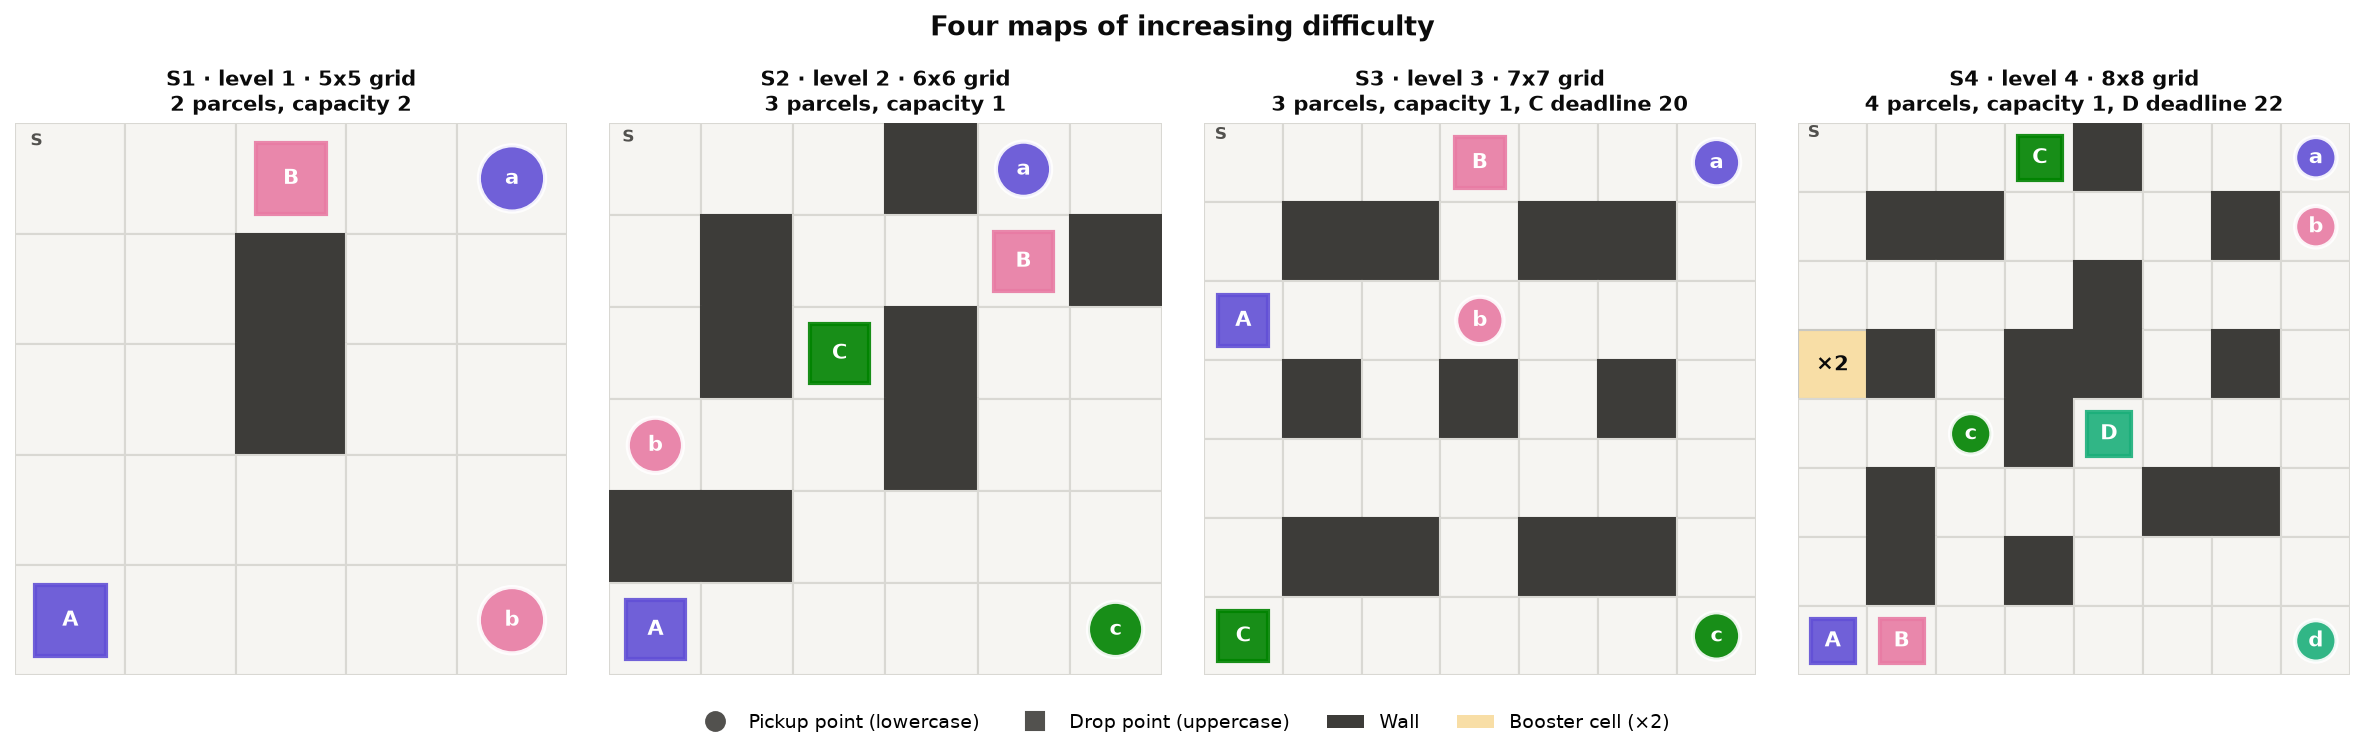
\includegraphics[width=\linewidth,height=0.62\textheight,keepaspectratio]{figures/fig02.png}
\caption{The four maps by level: pickup cells are circles (lowercase), drop cells are squares (uppercase), walls are dark, the ×2 booster cell is yellow}\label{fig:2}
\end{figure}

\begin{longtable}[]{@{}
  >{\raggedright\arraybackslash}p{(\columnwidth - 12\tabcolsep) * \real{0.1493}}
  >{\raggedright\arraybackslash}p{(\columnwidth - 12\tabcolsep) * \real{0.0728}}
  >{\raggedright\arraybackslash}p{(\columnwidth - 12\tabcolsep) * \real{0.0976}}
  >{\raggedright\arraybackslash}p{(\columnwidth - 12\tabcolsep) * \real{0.1151}}
  >{\raggedright\arraybackslash}p{(\columnwidth - 12\tabcolsep) * \real{0.2270}}
  >{\raggedright\arraybackslash}p{(\columnwidth - 12\tabcolsep) * \real{0.2085}}
  >{\raggedright\arraybackslash}p{(\columnwidth - 12\tabcolsep) * \real{0.1299}}@{}}
\caption{The four levels and their optimal routes (Value Iteration)}\label{tab:4}\\
\toprule\noalign{}
\begin{minipage}[b]{\linewidth}\raggedright
\textbf{Map}
\end{minipage} & \begin{minipage}[b]{\linewidth}\raggedright
\textbf{Grid}
\end{minipage} & \begin{minipage}[b]{\linewidth}\raggedright
\textbf{Parcels}
\end{minipage} & \begin{minipage}[b]{\linewidth}\raggedright
\textbf{Capacity}
\end{minipage} & \begin{minipage}[b]{\linewidth}\raggedright
\textbf{New mechanic}
\end{minipage} & \begin{minipage}[b]{\linewidth}\raggedright
\textbf{Optimal route}
\end{minipage} & \begin{minipage}[b]{\linewidth}\raggedright
\textbf{max\_steps}
\end{minipage} \\
\midrule\noalign{}
\endfirsthead
\caption[]{(continued)}\\
\toprule\noalign{}
\begin{minipage}[b]{\linewidth}\raggedright
\textbf{Map}
\end{minipage} & \begin{minipage}[b]{\linewidth}\raggedright
\textbf{Grid}
\end{minipage} & \begin{minipage}[b]{\linewidth}\raggedright
\textbf{Parcels}
\end{minipage} & \begin{minipage}[b]{\linewidth}\raggedright
\textbf{Capacity}
\end{minipage} & \begin{minipage}[b]{\linewidth}\raggedright
\textbf{New mechanic}
\end{minipage} & \begin{minipage}[b]{\linewidth}\raggedright
\textbf{Optimal route}
\end{minipage} & \begin{minipage}[b]{\linewidth}\raggedright
\textbf{max\_steps}
\end{minipage} \\
\midrule\noalign{}
\endhead
\bottomrule\noalign{}
\endlastfoot
S1 -- level 1 (easy) & 5x5 & 2 & 2 & Two independent parcels that can be
carried together & A → B: 22 steps, return 18 & 100 \\
S2 -- level 2 (medium) & 6x6 & 3 & 1 & Only 1 parcel at a time, so the
order matters & B → A → C: 36 steps, return 24 & 150 \\
S3 -- level 3 (hard) & 7x7 & 3 & 1 & Parcel C must be delivered within
the first 20 steps & C → B → A: 44 steps, return 16 & 200 \\
S4 -- level 4 (very hard) & 8x8 & 4 & 1 & Booster cell (carry 2 parcels
for one trip) and a 22-step deadline for parcel D & D → C → B → A with
the booster: 67 steps, return 13 & 300 \\
\end{longtable}

Difficulty grows on every measure: reachable states (186 → 535 → 4,027 →
15,612) and optimal route length (22 → 36 → 44 → 67 steps). S3 and S4
also require trade-offs. On S3, without the deadline the route B → A → C
would be 4 steps shorter, but the deadline forces the robot to deliver C
first. On S4 the robot must deliver D first to meet its deadline, then
detour via the booster cell to carry A and B in one trip, which saves 8
steps compared with no booster cell.

The "one trip" rule on S4: the booster trip starts when the robot enters
the booster cell and ends the first time the robot is empty-handed after
a Drop; the cell can be used only once per episode.

\hypertarget{algorithms}{%
\section{Algorithms}\label{algorithms}}

All three algorithms keep a Q table of size $|S|$ × 6 and
choose actions ε-greedily; they differ only in how the "target" used to
update Q is computed. All three train with exploring starts (Section
5.1).

\hypertarget{exploring-starts-and-the-ux3b5-greedy-policy}{%
\subsection{Exploring starts and the ε-greedy
policy}\label{exploring-starts-and-the-ux3b5-greedy-policy}}

\textbf{Exploring starts.} Every training episode starts in a randomly
chosen reachable state (parcels carried or delivered, any τ and b), and
the first action is also random. Every pair (s, a) is therefore updated
directly, including states such as "carrying C at τ = 15" that a robot
starting at τ = 0 rarely reaches. For evaluation the robot still starts
with every parcel waiting.

\textbf{ε-greedy.} After the first action, with probability ε one of the
6 actions is chosen at random, otherwise argmax Q(s, ·) (ties broken at
random). ε decays exponentially from ε\textsubscript{start} to
ε\textsubscript{end} over the first f·n\textsubscript{ep} episodes and
then stays constant; each algorithm has its own schedule (Table 5):

\[\varepsilon(ep) = \varepsilon_{start} \cdot \left( \frac{\varepsilon_{end}}{\varepsilon_{start}} \right)^{\min\left( 1,\frac{ep}{f \cdot n_{ep}} \right)}\]

Example: Q-learning on S3 (n\textsubscript{ep} = 2,000,000, ε: 1 → 0.01,
f = 0.8, so ε reaches its floor after 1,600,000 episodes), at episode
400,000:

\[\varepsilon = 1 \cdot \left( \frac{0.01}{1} \right)^{\frac{400,000}{1,600,000}} = {0.01}^{0.25} \approx 0.316\]

The final policy is the greedy policy: in every state it takes the
action with the largest Q. This policy is used for evaluation, for the
demo and for the policy figures:

\[\pi(s) = \underset{a}{arg\ max}{Q(s,a)}\]

\hypertarget{q-learning-off-policy-td}{%
\subsection{Q-learning (off-policy
TD)}\label{q-learning-off-policy-td}}

\[Q(s,a) \leftarrow Q(s,a) + \alpha\left\lbrack r + \gamma\max_{a'}{Q(s',a')} - Q(s,a) \right\rbrack\]

The update is applied after every step. The target depends on whether
that step really ends the episode:

\[\text{target} = \left\{ \begin{aligned}
 & r,\text{ if s' is terminal (all parcels delivered)} \\
 & r + \gamma\max_{a'}{Q(s',a')},\text{ otherwise}
\end{aligned} \right.\ \]

Being cut off by max\_steps is only a time limit, not a terminal state,
so the second case still applies. The environment is deterministic, so
the target has no noise and α = 1 can be used. Example with α = 1, γ =
0.99, Q(s,a) = 0, r = −1 and max Q(s′,a′) = 10:

\[\begin{aligned}
\text{target} & = r + \gamma\max_{a'}{Q(s',a')} = - 1 + 0.99 \cdot 10 = 8.9 \\
Q(s,a) & \leftarrow Q(s,a) + \alpha\left( \text{target} - Q(s,a) \right) = 0 + 1 \cdot (8.9 - 0) = 8.9
\end{aligned}\]

\hypertarget{sarsa-on-policy-td}{%
\subsection{SARSA (on-policy TD)}\label{sarsa-on-policy-td}}

\[Q(s,a) \leftarrow Q(s,a) + \alpha\left\lbrack r + \gamma Q(s',a') - Q(s,a) \right\rbrack\]

SARSA differs from Q-learning in exactly one place: max Q(s′, a′) is
replaced by Q(s′, a′), where a′ is the action the agent \textbf{will
actually take} in s′ (chosen ε-greedily, possibly an exploratory step).
SARSA therefore learns the value of the ε-greedy policy it is running
(on-policy) and only matches Q* as ε → 0. Same example as above, but in
s′ the agent draws an exploratory action with Q(s′, a′) = 2, and α =
0.5:

\[\begin{aligned}
\text{target} & = r + \gamma Q(s',a') = - 1 + 0.99 \cdot 2 = 0.98 \\
Q(s,a) & \leftarrow Q(s,a) + \alpha\left( \text{target} - Q(s,a) \right) = 0 + 0.5 \cdot (0.98 - 0) = 0.49
\end{aligned}\]

SARSA\textquotesingle s target is noisy because of the randomly drawn
action, so α cannot be 1: α decays linearly from 0.5 to 0.1. ε decays
exponentially to 10⁻⁵ during the first half of training, so the second
half is almost greedy (the GLIE condition: explore infinitely often but
become greedy in the limit).

\hypertarget{monte-carlo-es-on-policy}{%
\subsection{Monte Carlo ES
(on-policy)}\label{monte-carlo-es-on-policy}}

\[G_{t} = r_{t + 1} + \gamma G_{t + 1}\]

\[Q(s,a) \leftarrow Q(s,a) + \alpha\left\lbrack G_{t} - Q(s,a) \right\rbrack,\ \ \ \ \ \ \alpha = 1\]

The agent runs the whole episode, computes the returns backwards from
the end, and updates only the first occurrence of each pair (s, a)
(first-visit). Example with γ = 0.99 and last three rewards −1, −1 and
+19 (the delivery step gives −1 + 20 = +19):

\[\begin{aligned}
G_{T - 1} & = r_{T} = 19 \\
G_{T - 2} & = r_{T - 1} + \gamma G_{T - 1} = - 1 + 0.99 \cdot 19 = 17.81 \\
G_{T - 3} & = r_{T - 2} + \gamma G_{T - 2} = - 1 + 0.99 \cdot 17.81 = 16.63
\end{aligned}\]

The version used here is \textbf{Monte Carlo ES} (Sutton \& Barto,
Section 5.3): exploring starts for both s and a, then the greedy policy
(ε = 0), so all exploration comes from the random start. The environment
is deterministic and the policy greedy, so the return after (s, a) is a
fixed number for the current policy. α = 1 (Q equals the latest return)
is therefore used instead of the 1/N average, which would remember the
very negative returns of the early phase forever. If the policy loops,
the episode is cut at max\_steps with a very negative return, so the
action that caused the loop is penalised next time.

\hypertarget{settings-and-the-optimal-reference}{%
\subsection{Settings and the optimal
reference}\label{settings-and-the-optimal-reference}}

The training settings use full exploring starts, ε and α schedules
specific to each algorithm, more episodes (Table 5), and numba: the
environment is deterministic, so the transition function is precomputed
into three arrays NS, R, D, and the training loop only looks up these
arrays and is compiled to machine code, about 150--180 times faster.
Value Iteration (planner.py) iterates the Bellman optimality equation
over every reachable state to obtain the best return and Q*; it is not a
learning algorithm, only a reference:

\[V(s) = \max_{a}\left\lbrack r(s,a) + \gamma V(s') \right\rbrack\]

\begin{longtable}[]{@{}
  >{\raggedright\arraybackslash}p{(\columnwidth - 6\tabcolsep) * \real{0.2536}}
  >{\raggedright\arraybackslash}p{(\columnwidth - 6\tabcolsep) * \real{0.2488}}
  >{\raggedright\arraybackslash}p{(\columnwidth - 6\tabcolsep) * \real{0.2488}}
  >{\raggedright\arraybackslash}p{(\columnwidth - 6\tabcolsep) * \real{0.2488}}@{}}
\caption{Hyperparameters}\label{tab:5}\\
\toprule\noalign{}
\begin{minipage}[b]{\linewidth}\raggedright
\textbf{Hyperparameter}
\end{minipage} & \begin{minipage}[b]{\linewidth}\raggedright
\textbf{Q-learning}
\end{minipage} & \begin{minipage}[b]{\linewidth}\raggedright
\textbf{SARSA}
\end{minipage} & \begin{minipage}[b]{\linewidth}\raggedright
\textbf{Monte Carlo ES}
\end{minipage} \\
\midrule\noalign{}
\endfirsthead
\caption[]{(continued)}\\
\toprule\noalign{}
\begin{minipage}[b]{\linewidth}\raggedright
\textbf{Hyperparameter}
\end{minipage} & \begin{minipage}[b]{\linewidth}\raggedright
\textbf{Q-learning}
\end{minipage} & \begin{minipage}[b]{\linewidth}\raggedright
\textbf{SARSA}
\end{minipage} & \begin{minipage}[b]{\linewidth}\raggedright
\textbf{Monte Carlo ES}
\end{minipage} \\
\midrule\noalign{}
\endhead
\bottomrule\noalign{}
\endlastfoot
γ (discount) & \multicolumn{3}{l@{}}{%
0.99} \\
Step size α & 1 & 0.5 → 0.1 (linear decay) & 1 \\
ε & 1 → 0.01, exponential decay over the first 80\% & 1 → 10⁻⁵,
exponential decay over the first 50\% & 0 (always greedy) \\
Training start & \multicolumn{3}{l@{}}{%
Exploring starts: random reachable state and random first action} \\
Q₀ & \multicolumn{3}{l@{}}{%
0} \\
Episodes & \multicolumn{3}{l@{}}{%
S1: 100,000 · S2: 300,000 · S3: 2,000,000 · S4: 6,000,000} \\
Seeds & \multicolumn{3}{l@{}}{%
5 seeds (0--4) per algorithm} \\
Evaluation & \multicolumn{3}{l@{}}{%
200 times per training run: greedy policy (ε = 0) from S and from every
start cell} \\
\end{longtable}

\hypertarget{experimental-results}{%
\section{Experimental results}\label{experimental-results}}

All three algorithms reach \textbf{100\% accuracy on all 4 maps in 5/5
seeds} (60/60 runs): from every start cell, the greedy policy reaches
exactly the optimal return of Value Iteration. The difference is in
learning speed: Q-learning is the fastest, Monte Carlo ES second and
SARSA the slowest. Section 10 checks the harder case where the robot
starts in any reachable state.

Measurement: each training run is evaluated 200 times. Each evaluation
runs the greedy policy (ε = 0) from cell S (return, all parcels
delivered or not) and from every empty cell with every parcel waiting.
\textbf{Accuracy} is the percentage of start cells from which the policy
reaches exactly the optimal return of Value Iteration from that cell; it
is stricter than running from S only, where a policy could follow one
memorised route.

\begin{figure}[htbp]
\centering
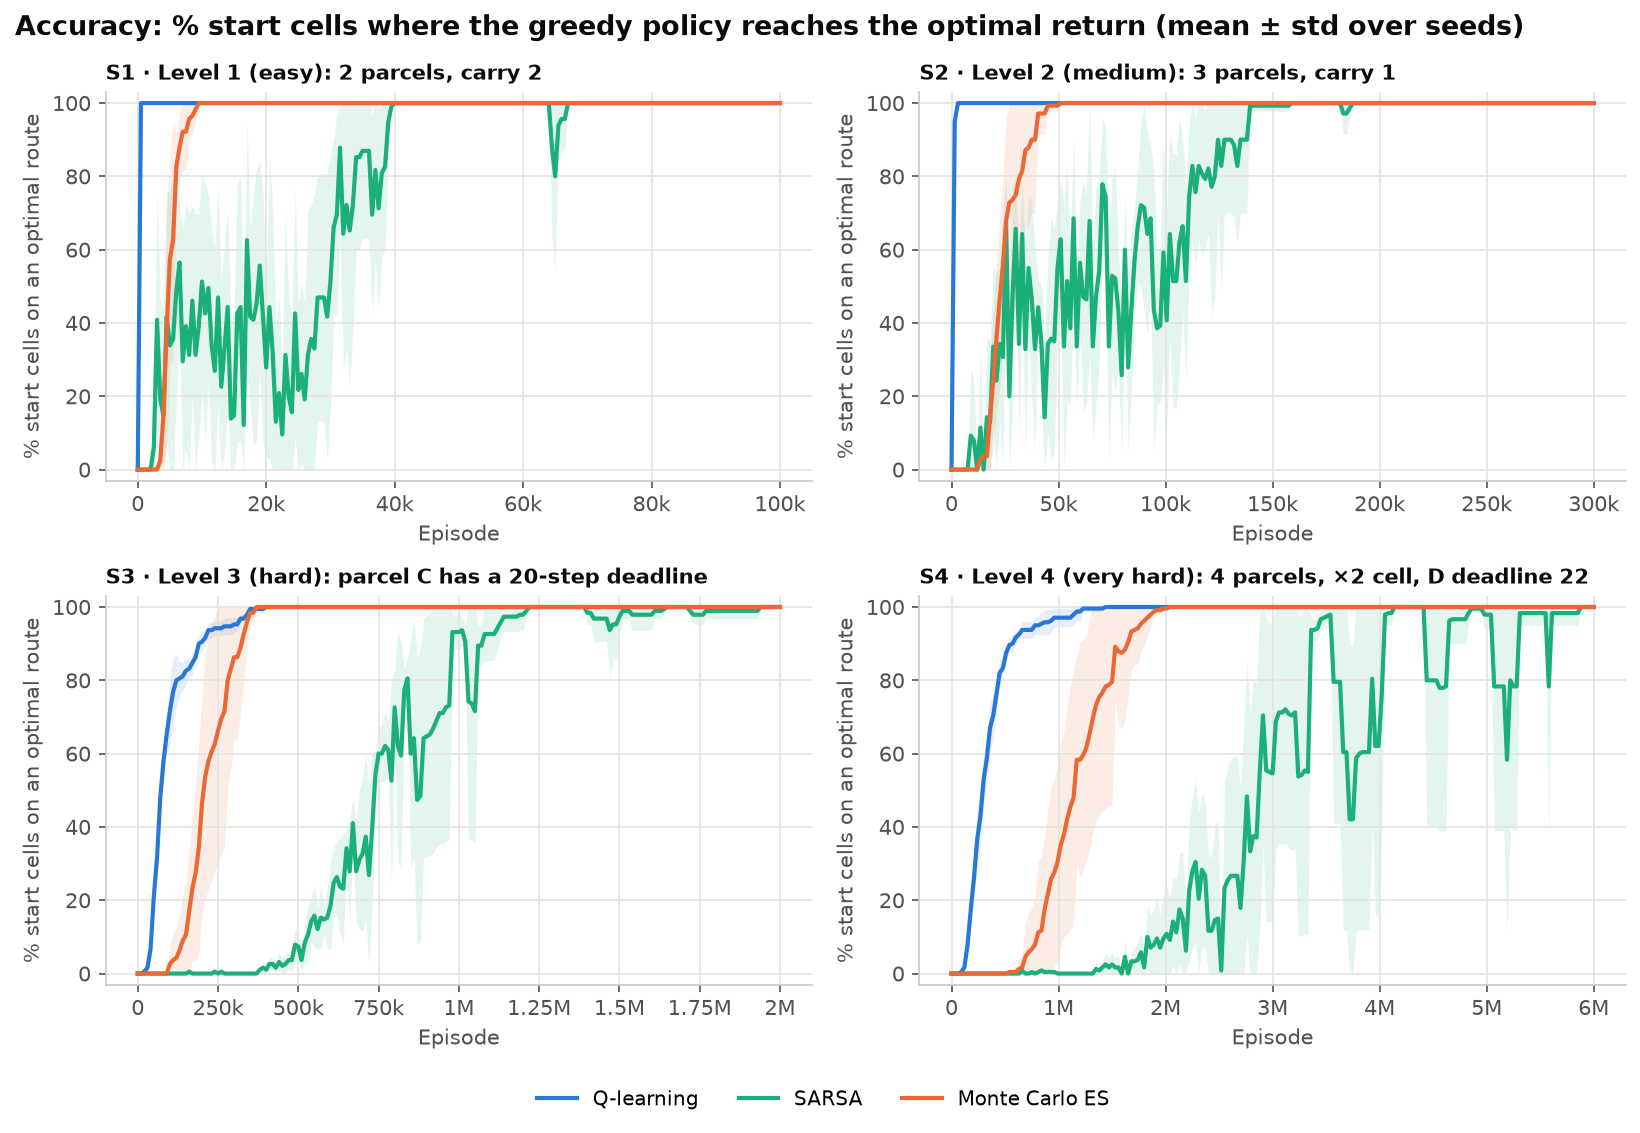
\includegraphics[width=\linewidth,height=0.62\textheight,keepaspectratio]{figures/fig03.png}
\caption{Accuracy over episodes: \% of start cells where the greedy policy reaches the optimal return, mean ± standard deviation over 5 seeds}\label{fig:3}
\end{figure}

\begin{longtable}[]{@{}
  >{\raggedright\arraybackslash}p{(\columnwidth - 10\tabcolsep) * \real{0.1433}}
  >{\raggedright\arraybackslash}p{(\columnwidth - 10\tabcolsep) * \real{0.1709}}
  >{\raggedright\arraybackslash}p{(\columnwidth - 10\tabcolsep) * \real{0.1268}}
  >{\raggedright\arraybackslash}p{(\columnwidth - 10\tabcolsep) * \real{0.1952}}
  >{\raggedright\arraybackslash}p{(\columnwidth - 10\tabcolsep) * \real{0.1213}}
  >{\raggedright\arraybackslash}p{(\columnwidth - 10\tabcolsep) * \real{0.2425}}@{}}
\caption{Final results (5 seeds)}\label{tab:6}\\
\toprule\noalign{}
\begin{minipage}[b]{\linewidth}\raggedright
\textbf{Map}
\end{minipage} & \begin{minipage}[b]{\linewidth}\raggedright
\textbf{Algorithm}
\end{minipage} & \begin{minipage}[b]{\linewidth}\raggedright
\textbf{Episodes}
\end{minipage} & \begin{minipage}[b]{\linewidth}\raggedright
\textbf{Return from S}
\end{minipage} & \begin{minipage}[b]{\linewidth}\raggedright
\textbf{Accuracy}
\end{minipage} & \begin{minipage}[b]{\linewidth}\raggedright
\textbf{First reaches 100\%}
\end{minipage} \\
\midrule\noalign{}
\endfirsthead
\caption[]{(continued)}\\
\toprule\noalign{}
\begin{minipage}[b]{\linewidth}\raggedright
\textbf{Map}
\end{minipage} & \begin{minipage}[b]{\linewidth}\raggedright
\textbf{Algorithm}
\end{minipage} & \begin{minipage}[b]{\linewidth}\raggedright
\textbf{Episodes}
\end{minipage} & \begin{minipage}[b]{\linewidth}\raggedright
\textbf{Return from S}
\end{minipage} & \begin{minipage}[b]{\linewidth}\raggedright
\textbf{Accuracy}
\end{minipage} & \begin{minipage}[b]{\linewidth}\raggedright
\textbf{First reaches 100\%}
\end{minipage} \\
\midrule\noalign{}
\endhead
\bottomrule\noalign{}
\endlastfoot
S1 (optimal 18) & Q-learning & 100,000 & 18 in all 5 seeds & 100\% &
500 \\
S1 & SARSA & 100,000 & 18 in all 5 seeds & 100\% & 5,500 -- 33,500 \\
S1 & Monte Carlo ES & 100,000 & 18 in all 5 seeds & 100\% & 7,000 --
9,500 \\
S2 (optimal 24) & Q-learning & 300,000 & 24 in all 5 seeds & 100\% &
1,500 -- 3,000 \\
S2 & SARSA & 300,000 & 24 in all 5 seeds & 100\% & 64,500 -- 159,000 \\
S2 & Monte Carlo ES & 300,000 & 24 in all 5 seeds & 100\% & 30,000 --
51,000 \\
S3 (optimal 16) & Q-learning & 2,000,000 & 16 in all 5 seeds, on time &
100\% & 340,000 -- 400,000 \\
S3 & SARSA & 2,000,000 & 16 in all 5 seeds, on time & 100\% & 980,000 --
1,220,000 \\
S3 & Monte Carlo ES & 2,000,000 & 16 in all 5 seeds, on time & 100\% &
260,000 -- 370,000 \\
S4 (optimal 13) & Q-learning & 6,000,000 & 13 in all 5 seeds, on time &
100\% & 840,000 -- 1,440,000 \\
S4 & SARSA & 6,000,000 & 13 in all 5 seeds, on time & 100\% & 3,450,000
-- 4,140,000 \\
S4 & Monte Carlo ES & 6,000,000 & 13 in all 5 seeds, on time & 100\% &
1,470,000 -- 2,040,000 \\
\end{longtable}

The Q tables also converge to Q*: the final mean error \textbar Q −
Q*\textbar{} is 0 for Q-learning and Monte Carlo ES and 0.001--0.05 for
SARSA (Figure 8). Time per seed on S4 (6 million episodes): Q-learning
38 s, SARSA 23 s, Monte Carlo ES 38 s.

\hypertarget{effect-of-the-number-of-episodes}{%
\subsection{Effect of the number of
episodes}\label{effect-of-the-number-of-episodes}}

Measured while tuning (same maps, same settings, 5 seeds). ε decays in
proportion to the number of episodes, so fewer episodes also means
shorter exploration.

\begin{longtable}[]{@{}
  >{\raggedright\arraybackslash}p{(\columnwidth - 4\tabcolsep) * \real{0.3000}}
  >{\raggedright\arraybackslash}p{(\columnwidth - 4\tabcolsep) * \real{0.3500}}
  >{\raggedright\arraybackslash}p{(\columnwidth - 4\tabcolsep) * \real{0.3500}}@{}}
\caption{Accuracy versus number of episodes}\label{tab:7}\\
\toprule\noalign{}
\begin{minipage}[b]{\linewidth}\raggedright
\textbf{Case}
\end{minipage} & \begin{minipage}[b]{\linewidth}\raggedright
\textbf{Fewer episodes}
\end{minipage} & \begin{minipage}[b]{\linewidth}\raggedright
\textbf{More episodes}
\end{minipage} \\
\midrule\noalign{}
\endfirsthead
\caption[]{(continued)}\\
\toprule\noalign{}
\begin{minipage}[b]{\linewidth}\raggedright
\textbf{Case}
\end{minipage} & \begin{minipage}[b]{\linewidth}\raggedright
\textbf{Fewer episodes}
\end{minipage} & \begin{minipage}[b]{\linewidth}\raggedright
\textbf{More episodes}
\end{minipage} \\
\midrule\noalign{}
\endhead
\bottomrule\noalign{}
\endlastfoot
S3, Q-learning & 200,000: 98.9\% & 2,000,000: 100\% \\
S3, Monte Carlo ES & 200,000: 46.3\% & 1,000,000: 100\% \\
S3, SARSA & 1,000,000: 99.5\% & 2,000,000: 100\% \\
S4, Q-learning & 500,000: 83.8\% & 2,000,000: 100\% \\
S4, Monte Carlo ES & 500,000: 0\%; 2,000,000: 99.6\% & 5,000,000:
100\% \\
S4, SARSA & 2,000,000: 41.2\% & 5,000,000: 99.6\%; 6,000,000: 100\% \\
\end{longtable}

SARSA needs the most episodes (about 3 times Q-learning on S4) because
it only learns Q* once ε is very small. To train even longer, run python
experiments.py -\/-scale 2.

\hypertarget{learned-policy-and-value-function}{%
\section{Learned policy and value
function}\label{learned-policy-and-value-function}}

The policy learned on S4 (Q-learning) matches the optimal solution: the
robot delivers parcel D first to meet its deadline, then detours via the
booster cell to carry two parcels in one trip, and finishes in 67 steps
with return 13.

How to read the figure: each small panel is one "phase" (a combination
of parcel statuses and booster status). Grey arrows show the action the
policy takes if the robot stands in that cell during this phase; P/D
mean Pickup/Drop. The coloured line is the actual route, coloured by the
parcel being carried: grey when empty-handed, black when carrying two
parcels.

\begin{figure}[htbp]
\centering
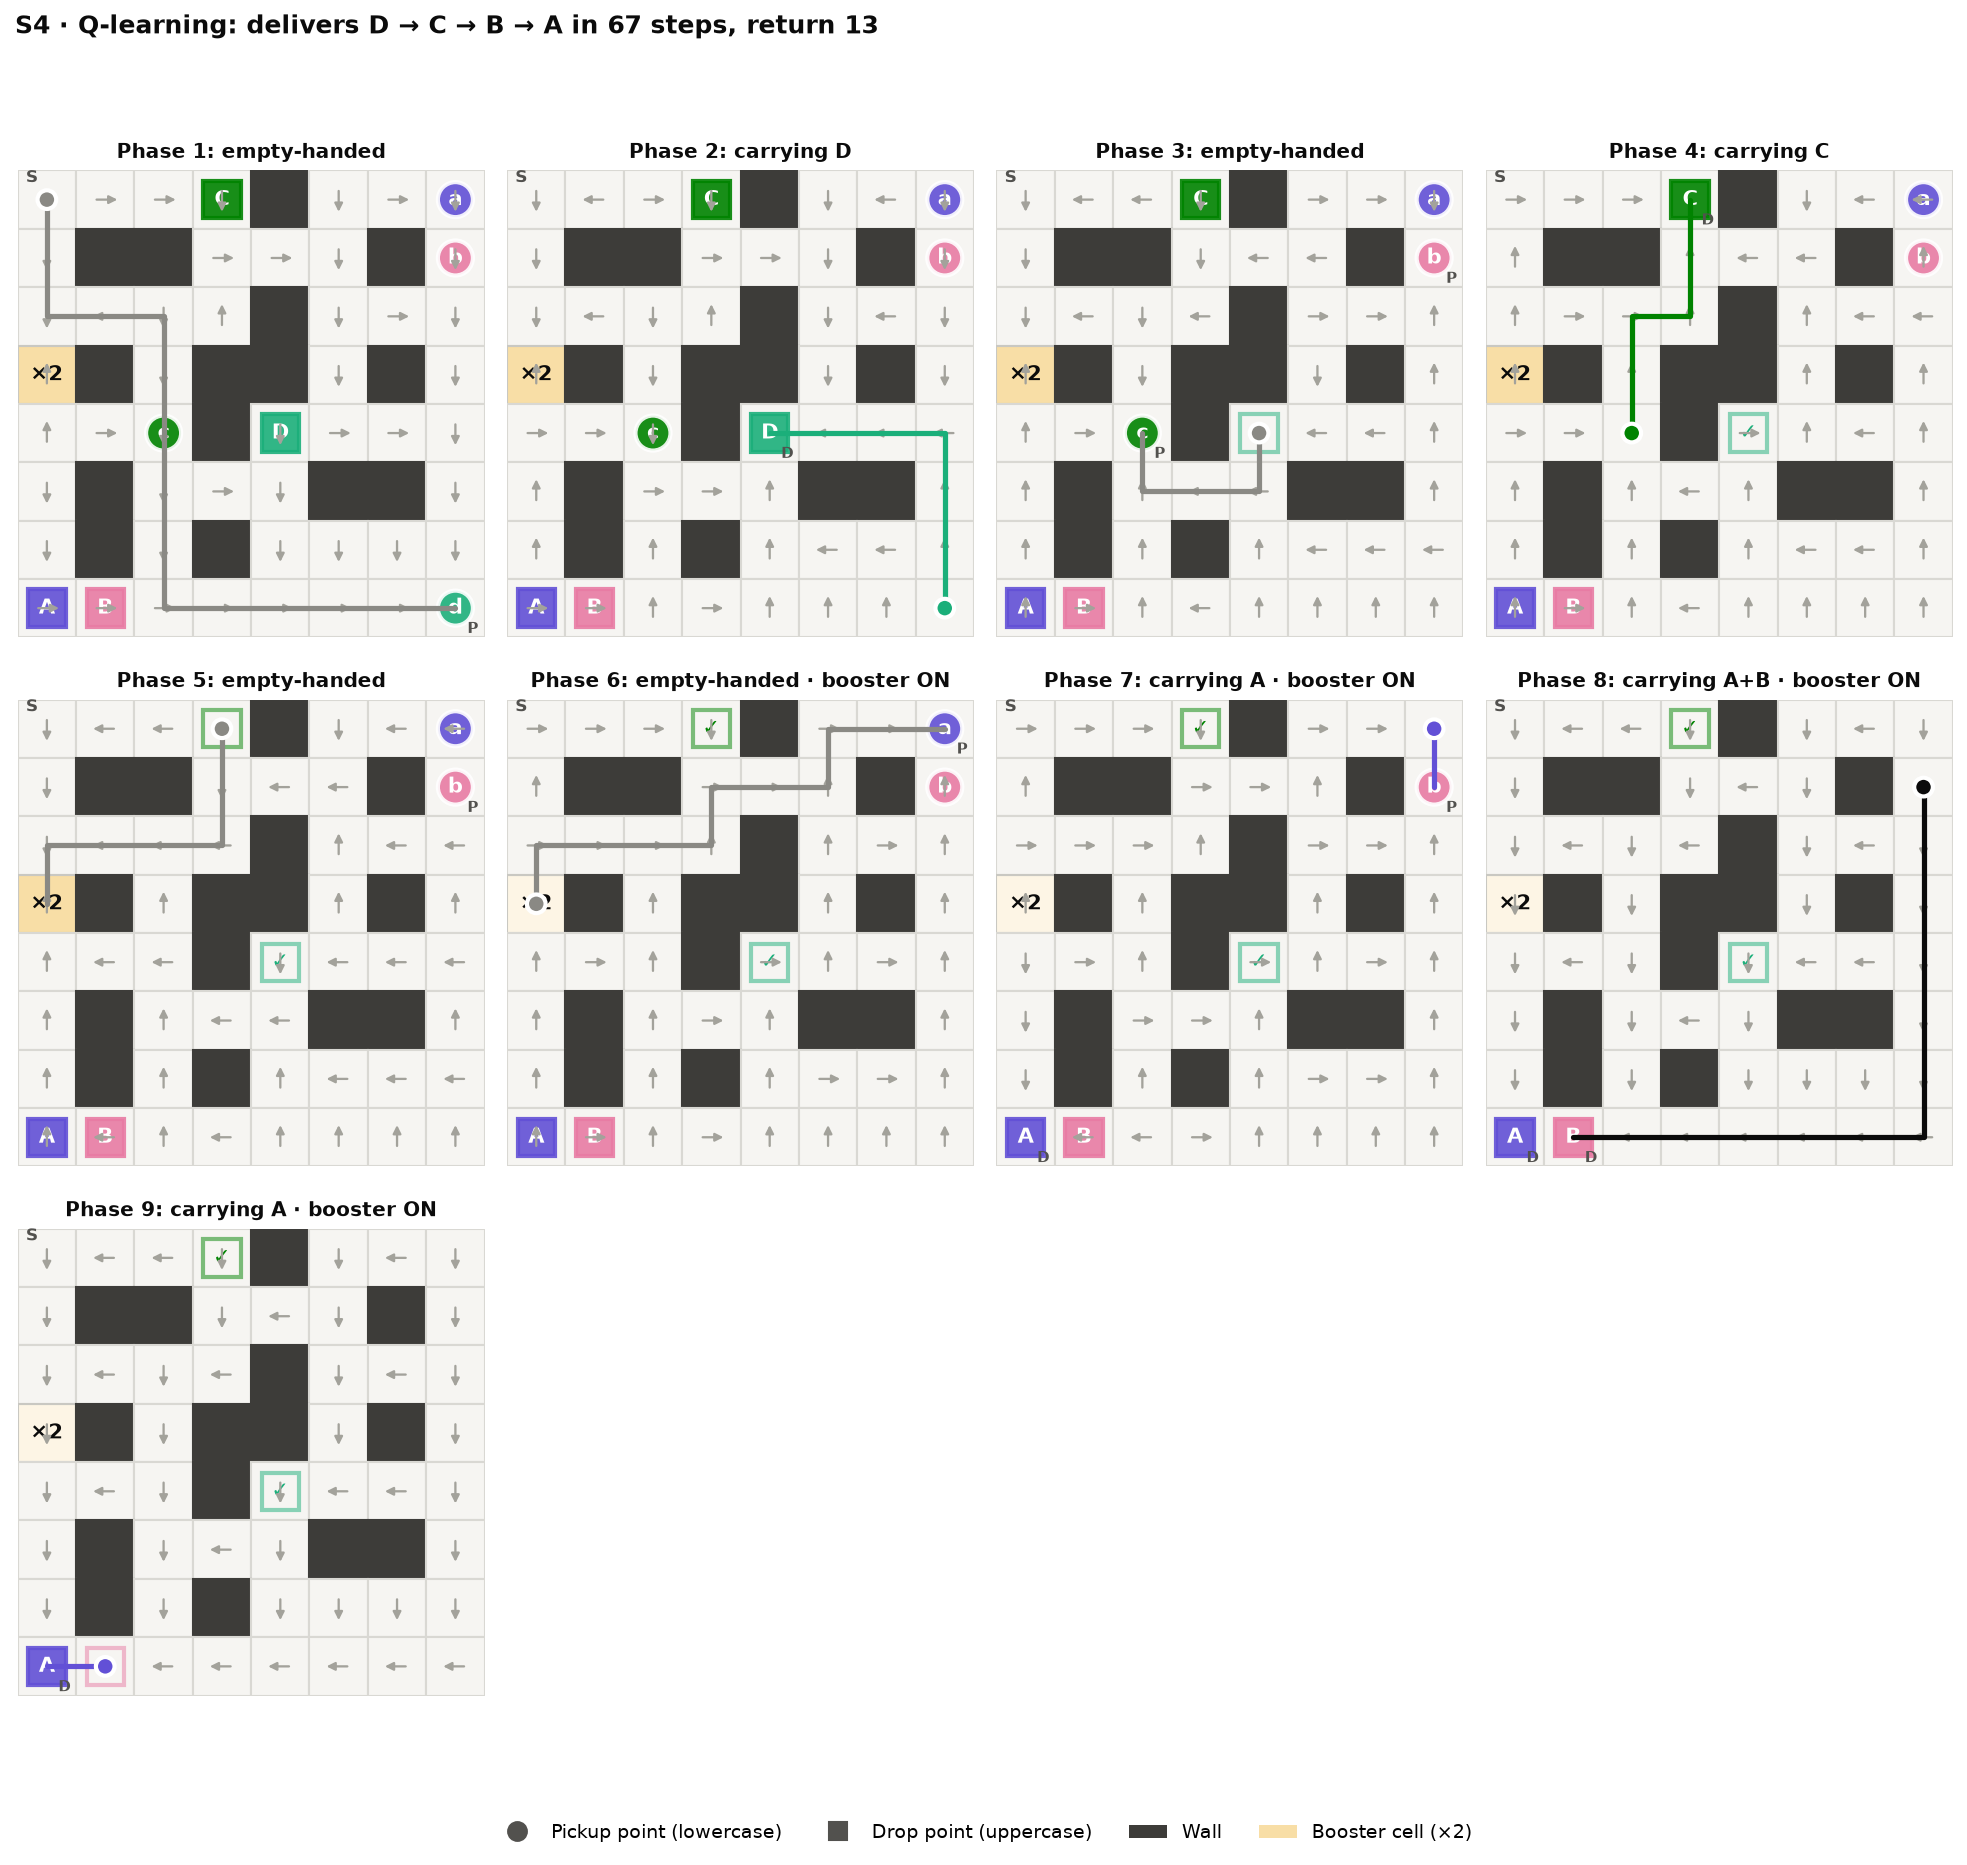
\includegraphics[width=\linewidth,height=0.62\textheight,keepaspectratio]{figures/fig04.png}
\caption{S4 policy (Q-learning): 9 phases from empty-handed to the last delivery}\label{fig:4}
\end{figure}

The sequence on S4:

\begin{enumerate}
\def\labelenumi{\arabic{enumi}.}
\item
  Pick up D in the bottom-right corner.
\item
  Deliver D in the middle of the map, before its 22-step deadline.
\item
  Pick up C, then deliver C on the top row.
\item
  Go down to the ×2 cell to switch the booster on.
\item
  Go to the top-right corner and pick up A, then B; the robot now
  carries A + B.
\item
  Carry both to the bottom-left corner and deliver B, then A.
\end{enumerate}

The agent learns both trade-offs by itself: it prioritises the deadline
parcel even though it is far away, and it accepts a detour to use the
booster cell.

\begin{figure}[htbp]
\centering
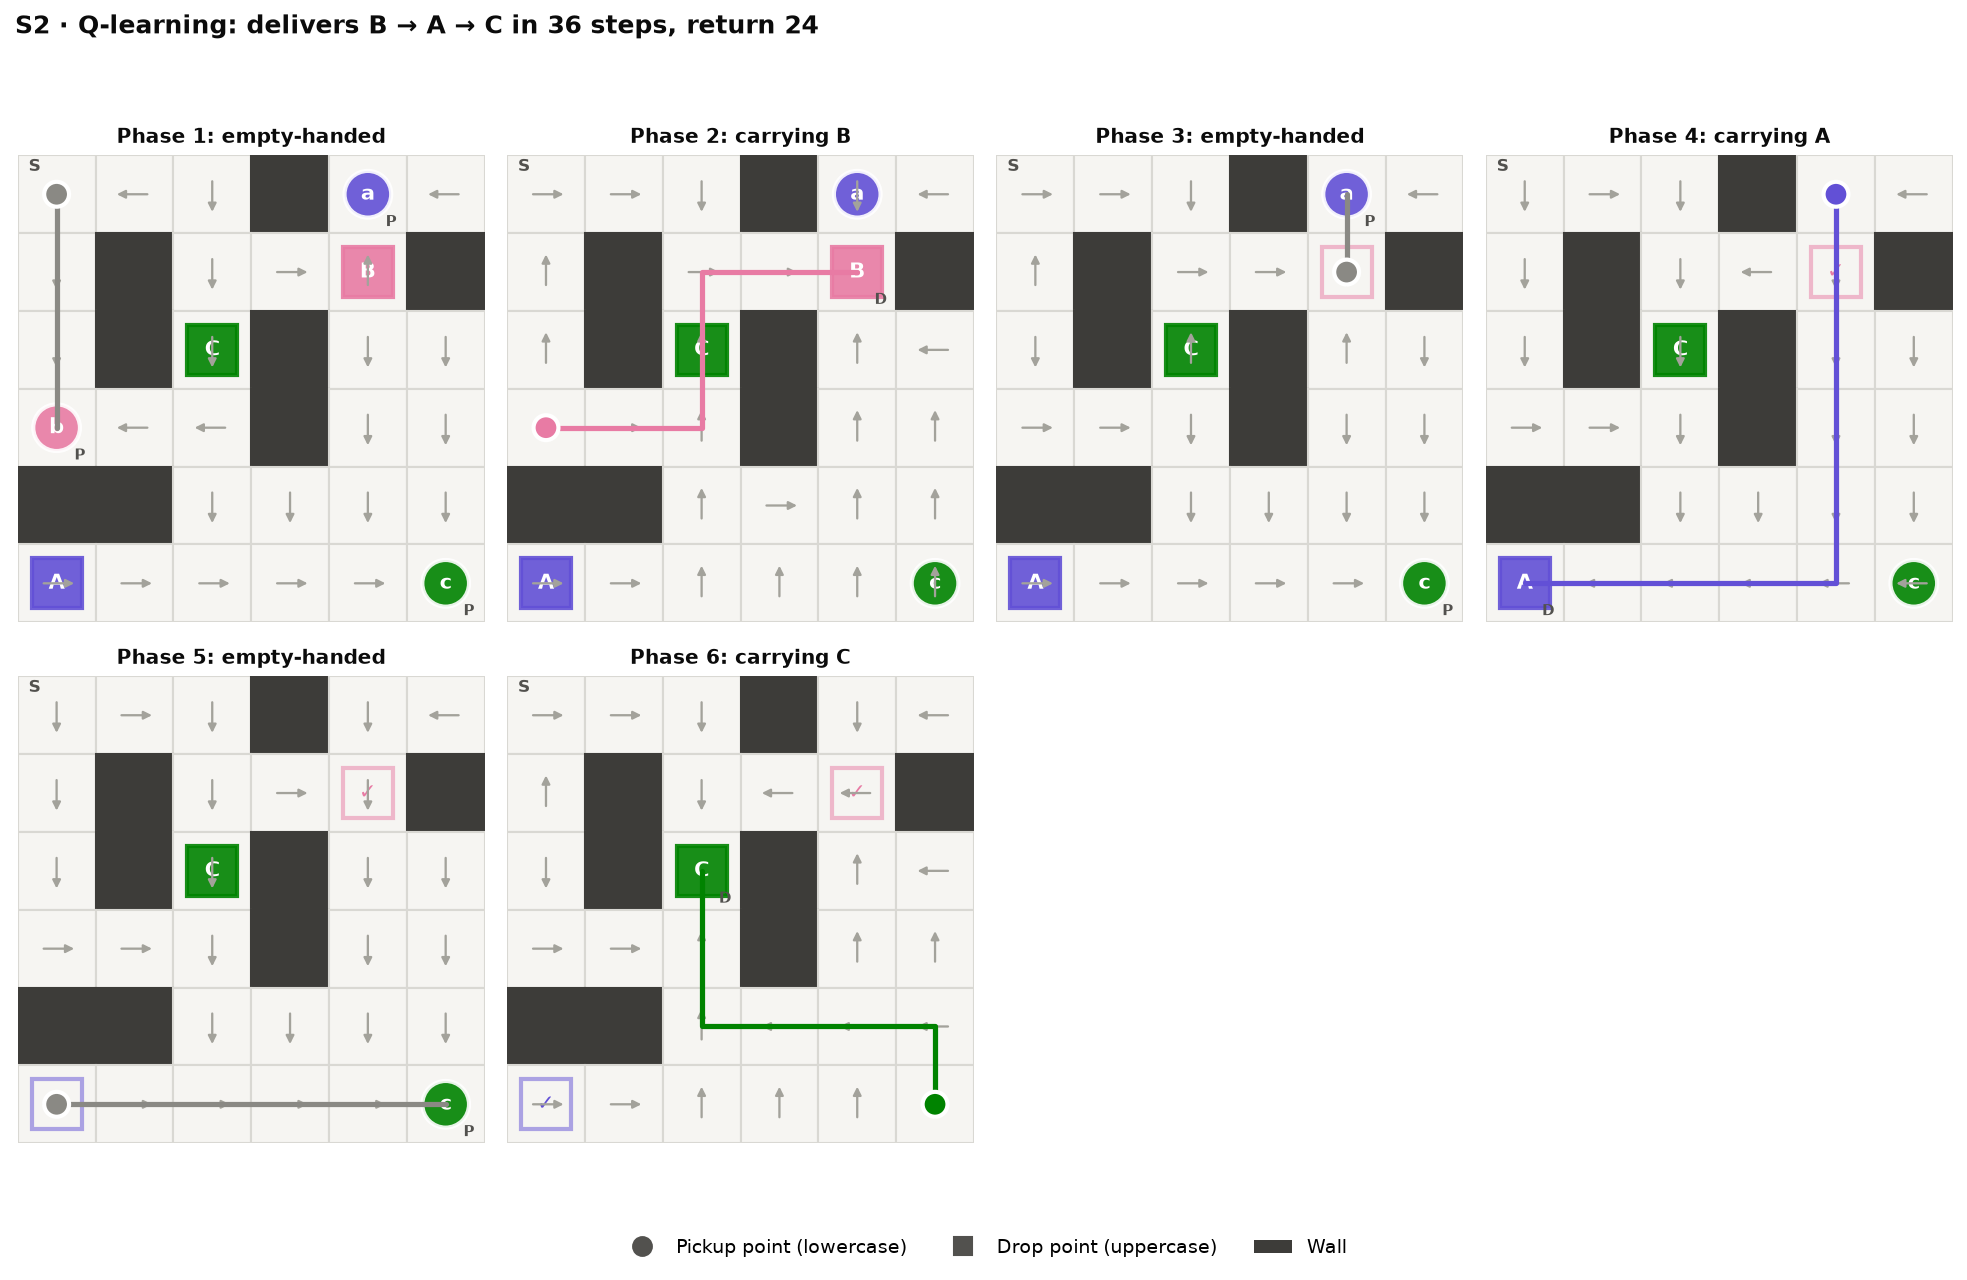
\includegraphics[width=\linewidth,height=0.62\textheight,keepaspectratio]{figures/fig05.png}
\caption{S2 policy (Q-learning): 6 phases, delivering B → A → C in 36 steps}\label{fig:5}
\end{figure}

On S2 the policy delivers in the order B → A → C (36 steps, return 24,
equal to the optimum). The arrows in cells off the route also point the
right way because exploring starts let the robot learn from every state.
figures\_en/policy\_S3.png shows the S3 policy in the same way.

\textbf{Value heatmaps.} Figure 6 colours every cell by the learned
value V(s) = max\textsubscript{a} Q(s, a) when the robot starts there
with every parcel waiting (τ = 0, b = 0): the darker the cell, the
higher the expected return. V at S is 13.7, 17.8, 8.6 and 2.5 for
S1--S4. These values are below the optimal returns (18, 24, 16 and 13)
because V is discounted with γ = 0.99, so a +20 reward collected late is
worth less.

\begin{figure}[htbp]
\centering
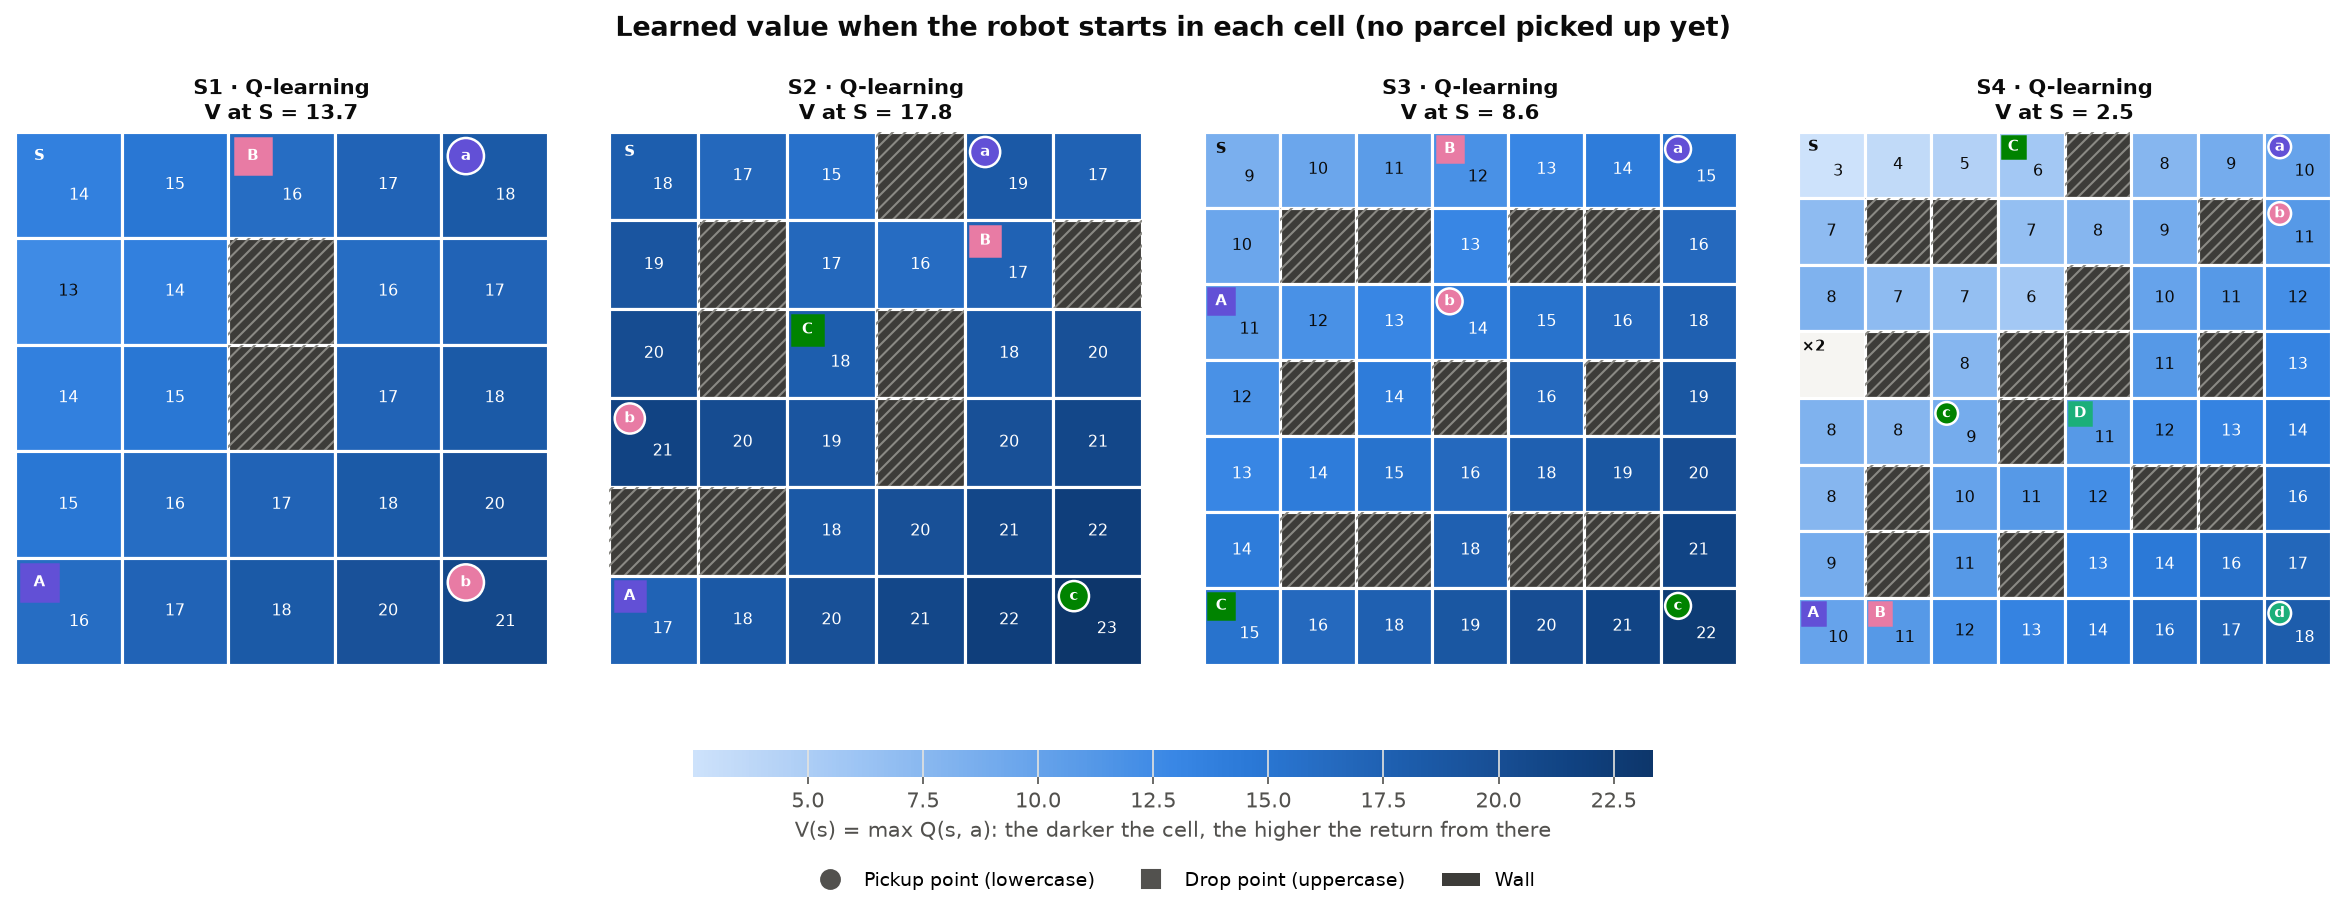
\includegraphics[width=\linewidth,height=0.62\textheight,keepaspectratio]{figures/fig06.png}
\caption{Learned start value V(s) = max Q(s, a) in every cell of the four maps (Q-learning, no parcel picked up yet); hatched cells are walls}\label{fig:6}
\end{figure}

Figure 7 repeats the heatmap for every phase of the S4 route, with the
same phases as Figure 4. Within a phase, cells close to the current
target (the parcel to pick up or the drop cell to reach) are darker, so
the greedy policy walks toward darker cells. The deadline is directly
visible: in phase 2 (carrying D, τ = 15) the cells far from
D\textquotesingle s drop cell fall to about −11, because from there D
can no longer arrive in time and the −30 penalty is certain. In phase 8
(carrying A and B thanks to the booster) almost the whole map is dark,
because two +20 rewards are only a few steps away. Phases that still
have a deadline are drawn at the τ of the start of the phase.

\begin{figure}[htbp]
\centering
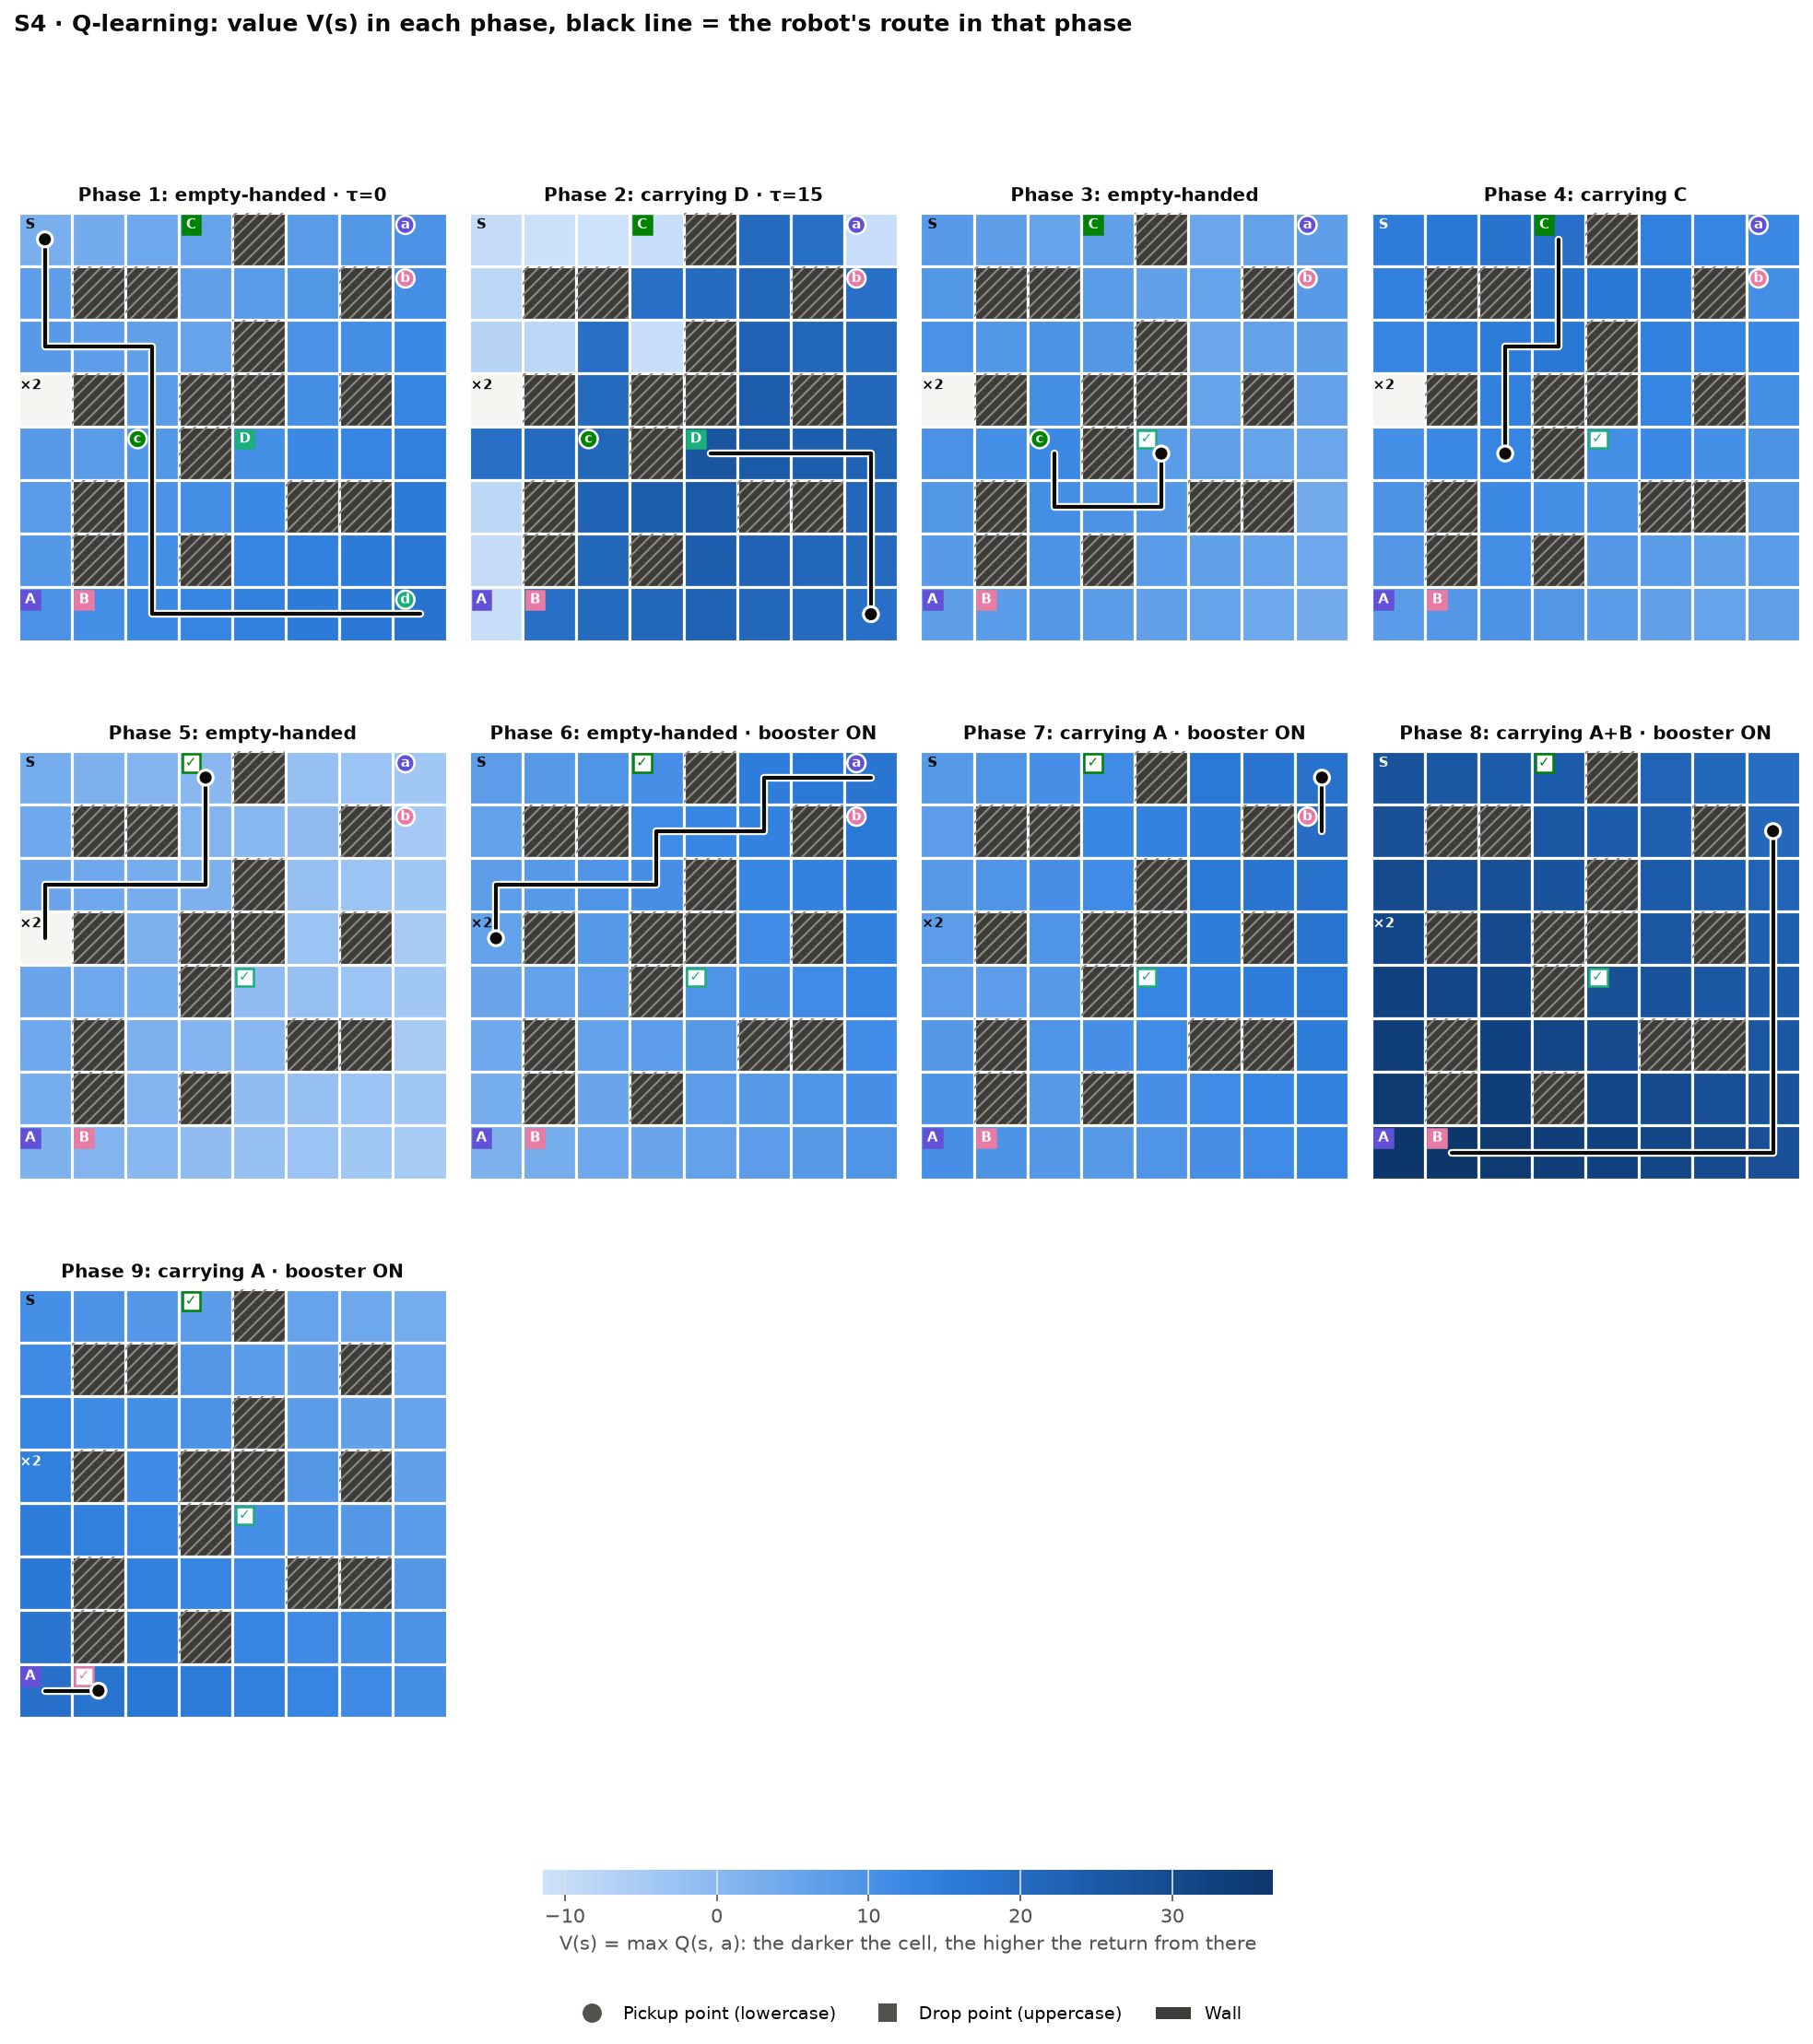
\includegraphics[width=0.80\linewidth,height=0.62\textheight,keepaspectratio]{figures/fig07.png}
\caption{S4 (Q-learning): learned value V(s) in each of the 9 phases; black line = the robot\textquotesingle s route in that phase}\label{fig:7}
\end{figure}

\hypertarget{comparing-the-three-algorithms}{%
\section{Comparing the three
algorithms}\label{comparing-the-three-algorithms}}

All three reach 100\%, so the comparison is about learning speed,
stability and sensitivity to settings (Table 8, Figure 8).

\begin{figure}[htbp]
\centering
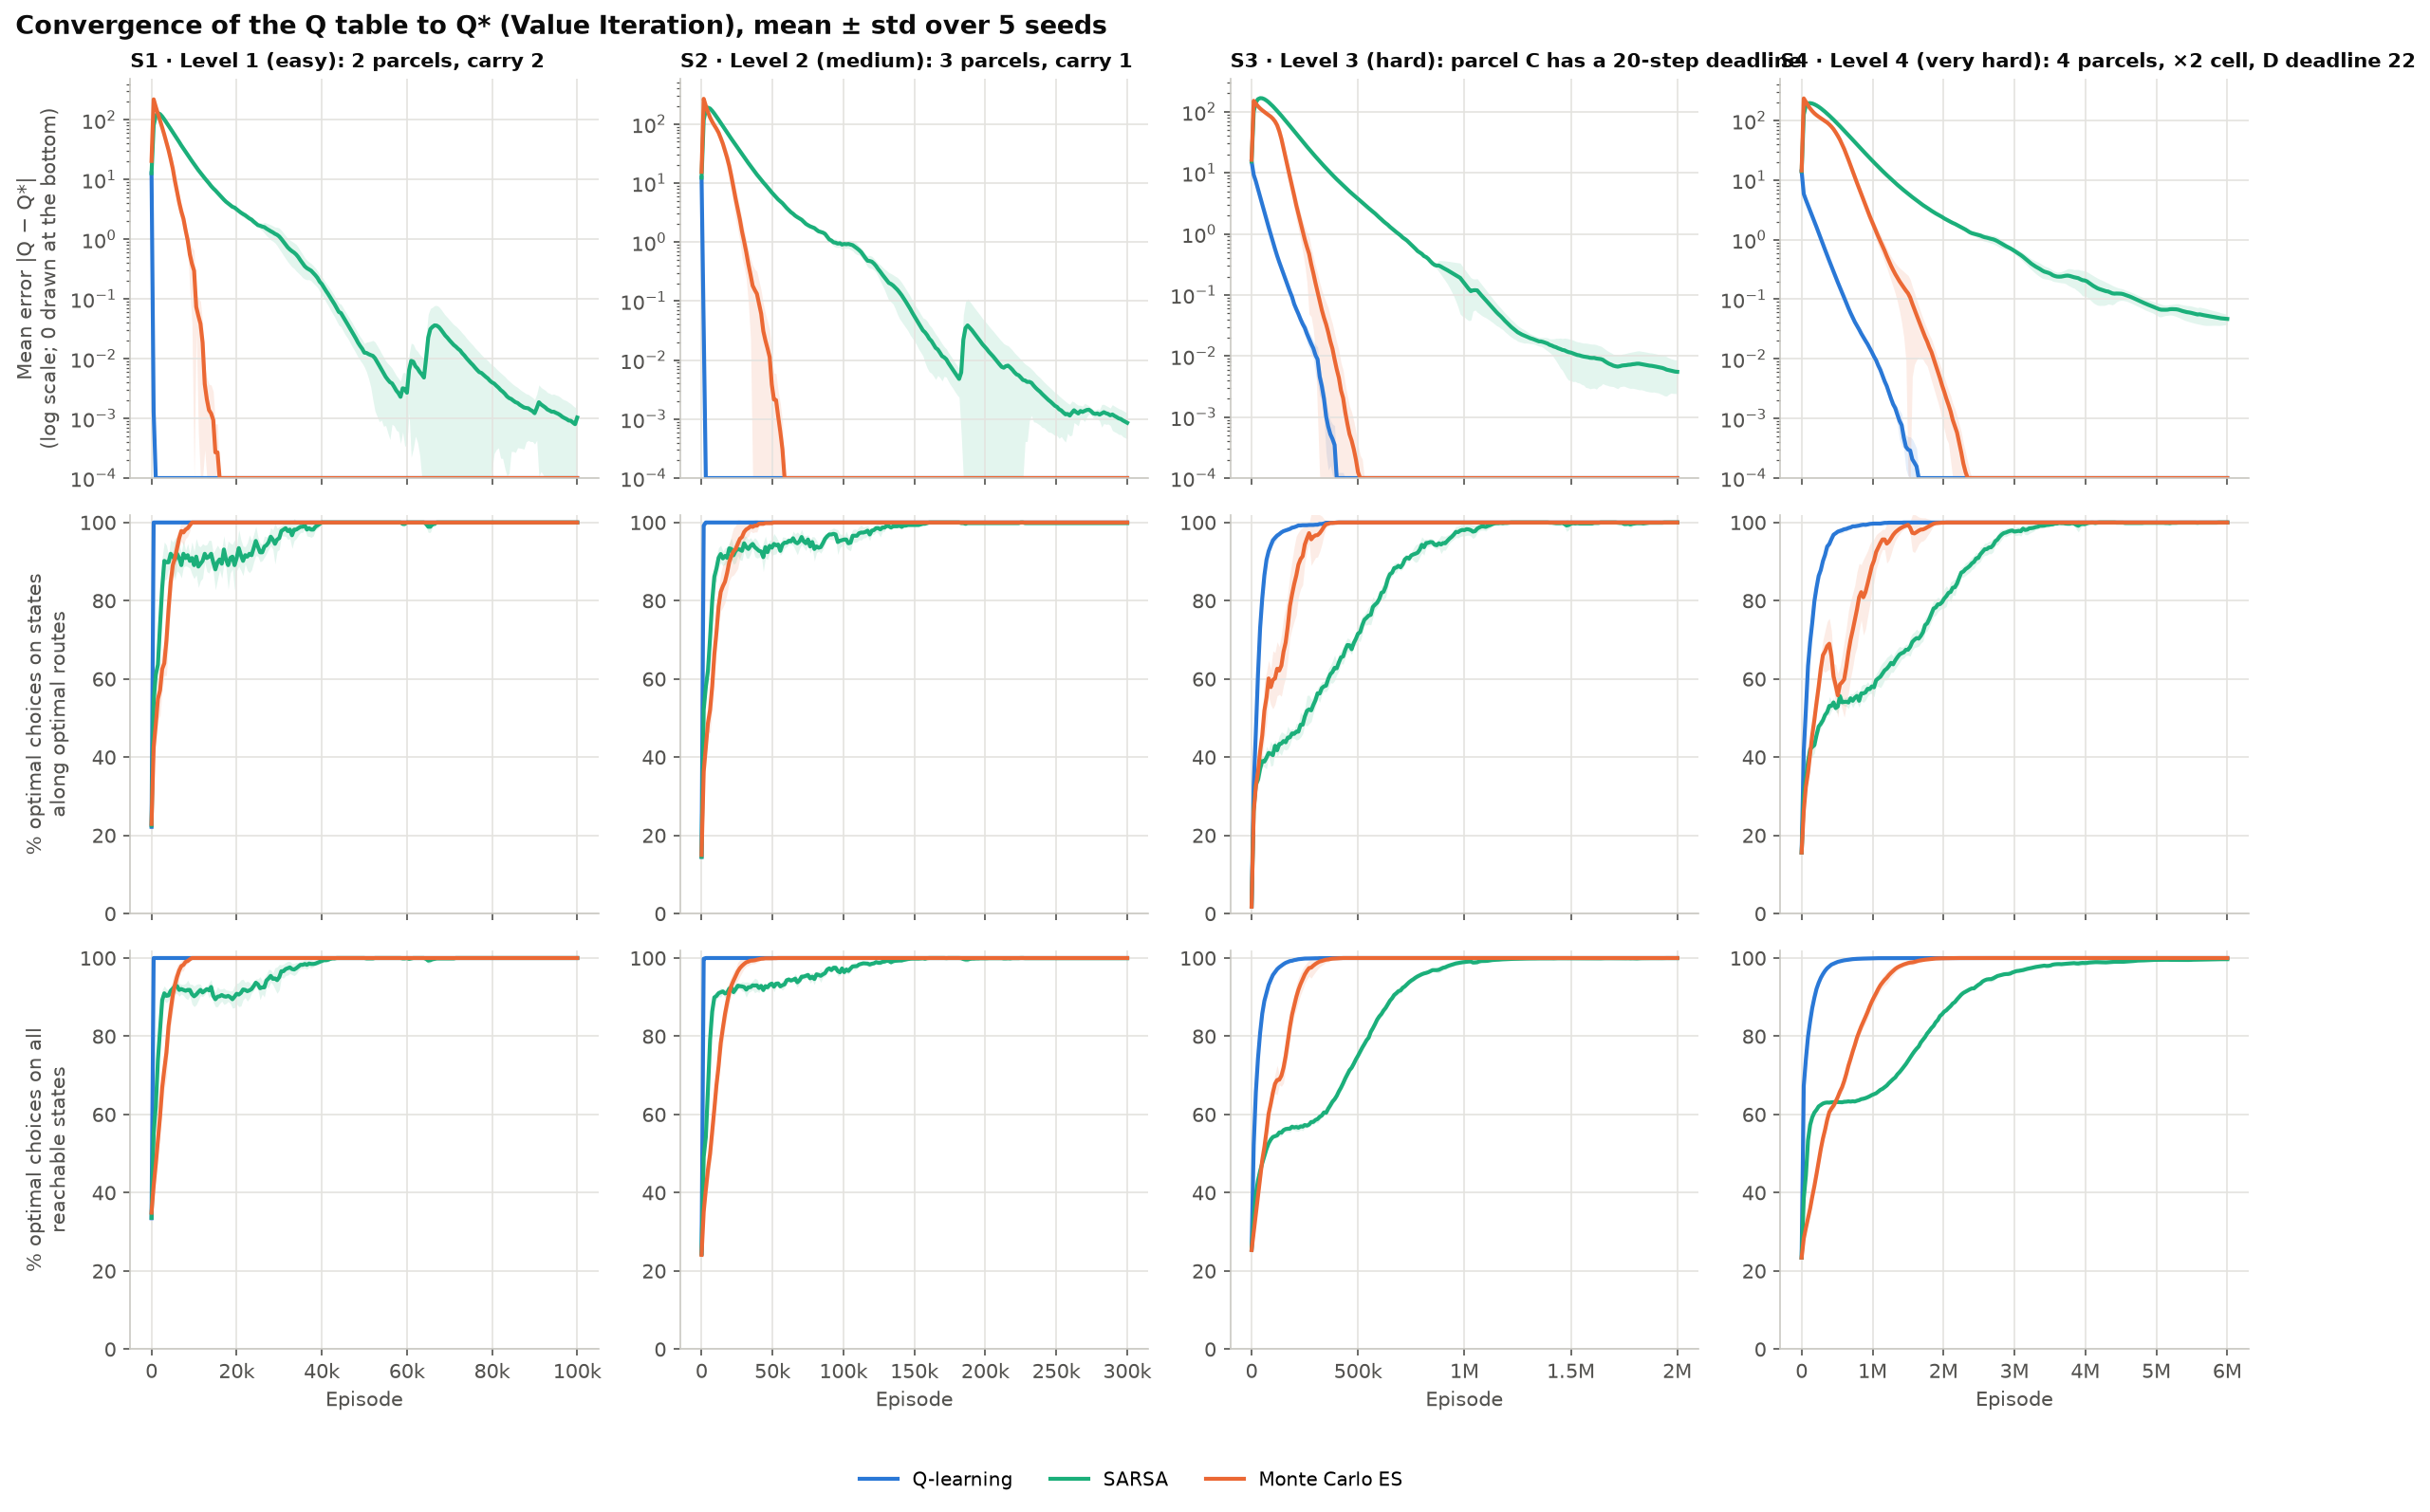
\includegraphics[width=\linewidth,height=0.62\textheight,keepaspectratio]{figures/fig08.png}
\caption{Convergence of the Q table to Q*: error \textbar Q − Q*\textbar{} (top row, log scale) and \% of states choosing the optimal action, mean ± standard deviation over 5 seeds}\label{fig:8}
\end{figure}

\begin{longtable}[]{@{}
  >{\raggedright\arraybackslash}p{(\columnwidth - 6\tabcolsep) * \real{0.2724}}
  >{\raggedright\arraybackslash}p{(\columnwidth - 6\tabcolsep) * \real{0.2425}}
  >{\raggedright\arraybackslash}p{(\columnwidth - 6\tabcolsep) * \real{0.2425}}
  >{\raggedright\arraybackslash}p{(\columnwidth - 6\tabcolsep) * \real{0.2425}}@{}}
\caption{Comparison of the three algorithms}\label{tab:8}\\
\toprule\noalign{}
\begin{minipage}[b]{\linewidth}\raggedright
\textbf{Criterion}
\end{minipage} & \begin{minipage}[b]{\linewidth}\raggedright
\textbf{Q-learning}
\end{minipage} & \begin{minipage}[b]{\linewidth}\raggedright
\textbf{SARSA}
\end{minipage} & \begin{minipage}[b]{\linewidth}\raggedright
\textbf{Monte Carlo ES}
\end{minipage} \\
\midrule\noalign{}
\endfirsthead
\caption[]{(continued)}\\
\toprule\noalign{}
\begin{minipage}[b]{\linewidth}\raggedright
\textbf{Criterion}
\end{minipage} & \begin{minipage}[b]{\linewidth}\raggedright
\textbf{Q-learning}
\end{minipage} & \begin{minipage}[b]{\linewidth}\raggedright
\textbf{SARSA}
\end{minipage} & \begin{minipage}[b]{\linewidth}\raggedright
\textbf{Monte Carlo ES}
\end{minipage} \\
\midrule\noalign{}
\endhead
\bottomrule\noalign{}
\endlastfoot
Update & After every step & After every step & After the whole
episode \\
Target & r + γ·max Q(s′), no noise & r + γ·Q(s′, a′), noisy through a′ &
Return G, no noise when ε = 0 \\
Learns the value of & The optimal policy (off-policy) & The ε-greedy
policy it runs (on-policy) & The current greedy policy (on-policy) \\
Episodes to 100\% on S4 (median) & 1,140,000 & 3,570,000 & 1,740,000 \\
Mean accuracy during training (S1 → S4) & 0.99 / 0.99 / 0.95 / 0.94 &
0.77 / 0.77 / 0.60 / 0.48 & 0.95 / 0.91 / 0.89 / 0.80 \\
Drops below 100\% after reaching it & Never & 9--19\% of measurements &
Never \\
Final error \textbar Q − Q*\textbar{} & 0 & 0.001 -- 0.047 & 0 \\
Wrong states when started anywhere (S3 / S4, Section 10) & 0 / 0 & 0.3\%
/ 1.8\% & 0 / 0 \\
Time per seed on S4 & 38 s & 23 s & 38 s \\
\end{longtable}

\textbf{Q-learning is the fastest and most stable.} Its target uses max
Q(s′), so it learns Q* directly from every step, including random
exploratory steps; the environment is deterministic, so the target has
no noise and α = 1 gives the exact value at once.

\textbf{Monte Carlo ES comes second.} It must wait for the end of the
episode before updating, so the early phase is slower, but a greedy
policy in a deterministic environment gives noise-free returns, so once
converged its Q is exactly right, like Q-learning. On S3 it even reaches
100\% earlier than Q-learning (290,000 versus 350,000 episodes, median)
because greedy training episodes are short. Its weakness is that it can
only learn thanks to exploring starts, its only source of exploration.

\textbf{SARSA is the slowest.} Its target uses the action it will
actually take, so SARSA learns the value of the exploring policy itself
and only matches Q* once ε is very small. The noisy target makes actions
with almost equal values swap back and forth, so the accuracy still
fluctuates after reaching 100\% and the Q table keeps a small error.
Section 10 shows what that small error does: started off its usual
route, SARSA takes a slightly longer route from 1.8\% of the S4 states.
Per second, though, a SARSA episode is the cheapest, because each step
chooses an action only once.

\textbf{Note.} SARSA\textquotesingle s usual advantage is behaving
safely while it still explores (for example in cliff walking); it does
not show here because the maps have no dangerous cells and a mistake
only costs −10. The ranking above holds for a deterministic environment;
if the robot\textquotesingle s wheels could slip, Q-learning and Monte
Carlo would lose the advantage of a noise-free target.

\hypertarget{reward-and-environment-parameter-experiments}{%
\section{Reward and environment-parameter
experiments}\label{reward-and-environment-parameter-experiments}}

All three changes alter the policy exactly as the optimal solution
predicts, in 5/5 seeds: removing the late penalty or relaxing the
deadline to 45 steps changes the delivery order from C → B → A to B → A
→ C, and removing the booster cell makes the route 8 steps longer. Each
variant uses Q-learning with the same number of episodes as the base
map.

\begin{longtable}[]{@{}
  >{\raggedright\arraybackslash}p{(\columnwidth - 4\tabcolsep) * \real{0.3400}}
  >{\raggedright\arraybackslash}p{(\columnwidth - 4\tabcolsep) * \real{0.3400}}
  >{\raggedright\arraybackslash}p{(\columnwidth - 4\tabcolsep) * \real{0.3200}}@{}}
\caption{Results of the reward / environment-parameter experiments}\label{tab:9}\\
\toprule\noalign{}
\begin{minipage}[b]{\linewidth}\raggedright
\textbf{Variant}
\end{minipage} & \begin{minipage}[b]{\linewidth}\raggedright
\textbf{Optimum (Value Iteration)}
\end{minipage} & \begin{minipage}[b]{\linewidth}\raggedright
\textbf{Learned by the agent (5 seeds)}
\end{minipage} \\
\midrule\noalign{}
\endfirsthead
\caption[]{(continued)}\\
\toprule\noalign{}
\begin{minipage}[b]{\linewidth}\raggedright
\textbf{Variant}
\end{minipage} & \begin{minipage}[b]{\linewidth}\raggedright
\textbf{Optimum (Value Iteration)}
\end{minipage} & \begin{minipage}[b]{\linewidth}\raggedright
\textbf{Learned by the agent (5 seeds)}
\end{minipage} \\
\midrule\noalign{}
\endhead
\bottomrule\noalign{}
\endlastfoot
S3 base: deadline 20, late penalty 30 & C → B → A, 44 steps, return 16 &
C → B → A, 44 steps, on time \\
S3: late penalty 30 → 0 & B → A → C, 40 steps, return 20 (late) & B → A
→ C, 40 steps \\
S3: deadline 20 → 45 & B → A → C, 40 steps, return 20 (on time) & B → A
→ C, 40 steps, on time \\
S4 base: with booster cell & D → C → B → A, 67 steps, return 13 & Same
as the optimum \\
S4: booster cell removed & D → B → C → A, 75 steps, return 5 & Same as
the optimum \\
\end{longtable}

\begin{figure}[htbp]
\centering
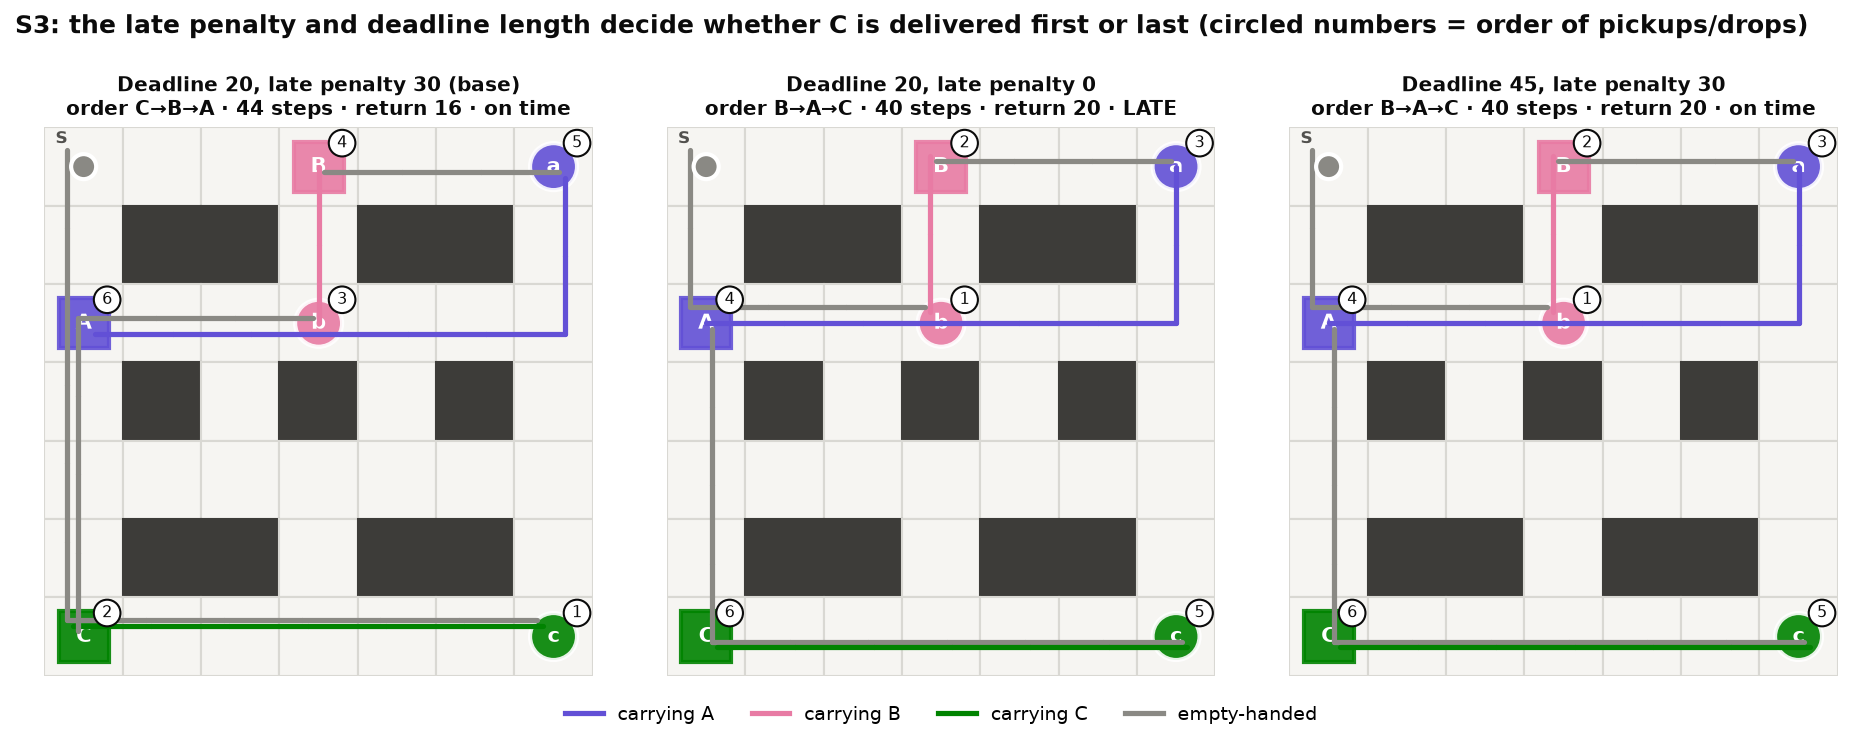
\includegraphics[width=\linewidth,height=0.62\textheight,keepaspectratio]{figures/fig09.png}
\caption{S3 with three configurations: the base delivers C first; late penalty 0 and deadline 45 both switch to B → A → C; circled numbers give the order of pickup/drop events}\label{fig:9}
\end{figure}

\textbf{Late penalty 30 → 0 (reward configuration).} When being late
costs nothing, B → A → C is 4 steps shorter, so the agent stops
prioritising parcel C and accepts a late delivery.

\textbf{Deadline 20 → 45 (environment parameter).} Delivering C last is
still on time, so the agent also switches to the shorter route B → A → C
without any penalty. The number of reachable states grows from 4,027 to
14,558, but Q-learning is still correct in 5/5 seeds.

\begin{figure}[htbp]
\centering
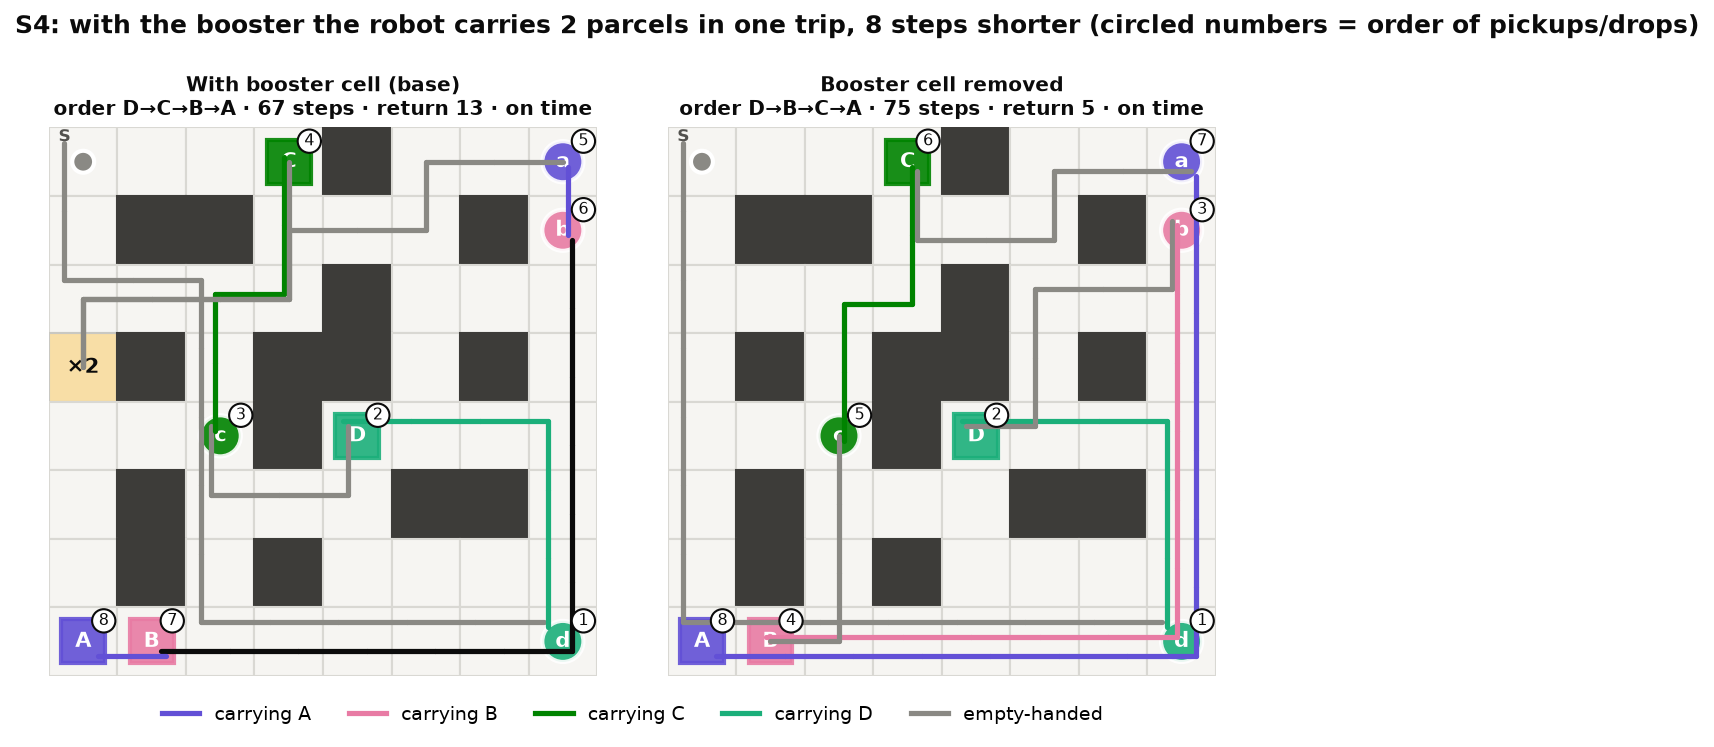
\includegraphics[width=0.90\linewidth,height=0.62\textheight,keepaspectratio]{figures/fig10.png}
\caption{S4 with and without the booster cell}\label{fig:10}
\end{figure}

\textbf{With / without the booster cell (environment parameter).}
Without the booster cell the robot needs four separate trips D → B → C →
A (75 steps). With it, the robot still delivers D first to meet its
deadline, delivers C, then detours via the ×2 cell to carry A and B
together (67 steps).

\hypertarget{when-does-the-robot-go-wrong}{%
\section{When does the robot go
wrong?}\label{when-does-the-robot-go-wrong}}

The accuracy of Section 6 starts the robot only in a start state: an
empty cell, every parcel waiting, τ = 0 and the booster unused. A policy
can be right there and still be wrong in states it seldom reaches: while
carrying a parcel, after some deliveries, with the deadline clock
running or with the booster on. Such states matter whenever the robot
does not begin a task from scratch, for example after it has been pushed
off its route or when it takes over a half-finished delivery.
failure\_cases.py therefore puts the robot in \textbf{every reachable
state that is not finished yet} (184 states on S1 up to 15,604 on S4),
runs the greedy policy from there and compares its return with the
return of Value Iteration from the same state.

Three groups of runs are checked, 5 seeds each: the settings of Section
5.5 on all four maps, and on S3 and S4 two SARSA variants: twice as many
episodes, and a final step size α = 0.02 instead of 0.1. Seed 0 uses the
Q tables saved by experiments.py; every other run is retrained with the
same seed, which reproduces the runs of Section 6 exactly because
training is deterministic for a given seed. Checking one Q table takes
less than a second.

\hypertarget{how-a-mistake-is-classified}{%
\subsection{How a mistake is
classified}\label{how-a-mistake-is-classified}}

A state is \textbf{wrong} when the greedy policy collects less than the
optimal return from it. Each wrong state gets exactly one type, checked
in the order of Table 10. This measure counts what a mistake costs over
the rest of the episode. It differs from the share of states whose
greedy action is not optimal (bottom row of Figure 8): an action that
differs from Value Iteration\textquotesingle s but leads to an equally
short route is not counted as a mistake here.

\begin{longtable}[]{@{}
  >{\raggedright\arraybackslash}p{(\columnwidth - 4\tabcolsep) * \real{0.2095}}
  >{\raggedright\arraybackslash}p{(\columnwidth - 4\tabcolsep) * \real{0.5701}}
  >{\raggedright\arraybackslash}p{(\columnwidth - 4\tabcolsep) * \real{0.2205}}@{}}
\caption{Types of mistakes, checked in this order}\label{tab:10}\\
\toprule\noalign{}
\begin{minipage}[b]{\linewidth}\raggedright
\textbf{Type}
\end{minipage} & \begin{minipage}[b]{\linewidth}\raggedright
\textbf{What the robot does}
\end{minipage} & \begin{minipage}[b]{\linewidth}\raggedright
\textbf{Cost}
\end{minipage} \\
\midrule\noalign{}
\endfirsthead
\caption[]{(continued)}\\
\toprule\noalign{}
\begin{minipage}[b]{\linewidth}\raggedright
\textbf{Type}
\end{minipage} & \begin{minipage}[b]{\linewidth}\raggedright
\textbf{What the robot does}
\end{minipage} & \begin{minipage}[b]{\linewidth}\raggedright
\textbf{Cost}
\end{minipage} \\
\midrule\noalign{}
\endhead
\bottomrule\noalign{}
\endlastfoot
\textbf{Never finishes} & max\_steps runs out with parcels left. The
policy and the environment are deterministic, so once the robot is back
in a state it has already visited it repeats the same cycle forever & −1
per remaining step \\
\textbf{Late} & Pays the late penalty although the optimal route from
the same state is on time & 30 or more \\
\textbf{Illegal action} & Makes at least one Pickup or Drop in the wrong
cell & 10 or more per action \\
\textbf{Longer route} & Delivers everything, on time and without illegal
actions, but with more steps than the optimal route & 1 per extra
step \\
\end{longtable}

Every state has a \textbf{state code}: the integer idx = encode(s) of
Section 3, which is also the row of the Q table. For each wrong state,
failure\_cases.py also follows the greedy route to the first state whose
greedy action is not optimal under Q*; this \textbf{wrong decision} is
where the robot actually turns the wrong way, and it can lie several
steps after the start state. Every wrong state is written to
results/failure\_states.csv with its state code, the decoded tuple s =
(row, col, σ₁, \ldots, σ\textsubscript{N}, τ, b), the type of mistake,
the points lost, and the state code, tuple and actions of its wrong
decision. In the code, rollout() runs the greedy policy from all states
at once through the tables NS, R, D, analyse() classifies the mistakes,
decisions() finds the wrong decisions and write\_states() writes the CSV
file. The core of the search for the wrong decision is shown below
(comments translated, slightly shortened); Appendix A lists every wrong
decision of SARSA with its state code.

\begin{lstlisting}
# in analyse(): S = all reachable unfinished states, Qs = Q*
a = Q[S].argmax(axis=1)                         # greedy action of Q
wrong = np.zeros(env.n_states, dtype=bool)
wrong[S] = Qs[S, a] < Qs[S].max(axis=1) - 1e-6   # not optimal in Q*
\end{lstlisting}

\begin{lstlisting}
def decisions(env, Q, wrong, starts):            # failure_cases.py
    NS, _, D = env.tables()
    cur = np.asarray(starts, dtype=np.int64).copy()
    dec = np.full(len(cur), -1)                  # wrong-decision code
    dist = np.zeros(len(cur), dtype=np.int64)
    live = np.ones(len(cur), dtype=bool)
    for _ in range(env.max_steps):
        hit = live & wrong[cur]                  # first wrong action
        dec[hit] = cur[hit]
        live &= ~hit
        if not live.any():
            break
        act = Q[cur].argmax(axis=1)              # follow the greedy route
        live &= ~D[cur, act]
        cur = np.where(live, NS[cur, act], cur)
        dist += live                             # steps before it
    return dec, dist
\end{lstlisting}

\hypertarget{started-in-every-reachable-state}{%
\subsection{Started in every reachable
state}\label{started-in-every-reachable-state}}

\textbf{Q-learning and Monte Carlo ES are right in every reachable
state} on all four maps, in all 5 seeds (Table 11). This agrees with
Figure 8: their Q tables equal Q*. SARSA is right everywhere on S1 and
S2, but takes a longer route from 0--46 of the 4,024 states on S3 (0.3\%
on average) and from 273--301 of the 15,604 states on S4 (1.8\%). Every
one of these SARSA mistakes is a longer route: no loop, no late delivery
and no illegal action, and the robot loses at most 6 points (6 extra
steps). From the start states SARSA is still 100\% correct, which is why
Section 6 cannot see these mistakes.

\begin{longtable}[]{@{}
  >{\raggedright\arraybackslash}p{(\columnwidth - 10\tabcolsep) * \real{0.1952}}
  >{\raggedright\arraybackslash}p{(\columnwidth - 10\tabcolsep) * \real{0.1323}}
  >{\raggedright\arraybackslash}p{(\columnwidth - 10\tabcolsep) * \real{0.1874}}
  >{\raggedright\arraybackslash}p{(\columnwidth - 10\tabcolsep) * \real{0.1433}}
  >{\raggedright\arraybackslash}p{(\columnwidth - 10\tabcolsep) * \real{0.1709}}
  >{\raggedright\arraybackslash}p{(\columnwidth - 10\tabcolsep) * \real{0.1709}}@{}}
\caption{Number of wrong states per seed (range over 5 seeds; mean share in brackets)}\label{tab:11}\\
\toprule\noalign{}
\begin{minipage}[b]{\linewidth}\raggedright
\textbf{Map (reachable states)}
\end{minipage} & \begin{minipage}[b]{\linewidth}\raggedright
\textbf{Q-learning}
\end{minipage} & \begin{minipage}[b]{\linewidth}\raggedright
\textbf{SARSA}
\end{minipage} & \begin{minipage}[b]{\linewidth}\raggedright
\textbf{Monte Carlo ES}
\end{minipage} & \begin{minipage}[b]{\linewidth}\raggedright
\textbf{SARSA, 2× episodes}
\end{minipage} & \begin{minipage}[b]{\linewidth}\raggedright
\textbf{SARSA, final α 0.02}
\end{minipage} \\
\midrule\noalign{}
\endfirsthead
\caption[]{(continued)}\\
\toprule\noalign{}
\begin{minipage}[b]{\linewidth}\raggedright
\textbf{Map (reachable states)}
\end{minipage} & \begin{minipage}[b]{\linewidth}\raggedright
\textbf{Q-learning}
\end{minipage} & \begin{minipage}[b]{\linewidth}\raggedright
\textbf{SARSA}
\end{minipage} & \begin{minipage}[b]{\linewidth}\raggedright
\textbf{Monte Carlo ES}
\end{minipage} & \begin{minipage}[b]{\linewidth}\raggedright
\textbf{SARSA, 2× episodes}
\end{minipage} & \begin{minipage}[b]{\linewidth}\raggedright
\textbf{SARSA, final α 0.02}
\end{minipage} \\
\midrule\noalign{}
\endhead
\bottomrule\noalign{}
\endlastfoot
S1 (184) & 0 & 0 & 0 & -- & -- \\
S2 (532) & 0 & 0 & 0 & -- & -- \\
S3 (4,024) & 0 & 0--46 (0.3\%) & 0 & 0--41 (0.3\%) & 0 \\
S4 (15,604) & 0 & 273--301 (1.8\%) & 0 & 144--413 (1.8\%) & 29--283
(0.9\%) \\
\end{longtable}

\hypertarget{a-typical-sarsa-mistake}{%
\subsection{A typical SARSA
mistake}\label{a-typical-sarsa-mistake}}

Figure 11 shows the costliest state of SARSA seed 0 on S4. The robot is
in the top-left corner, carries parcel C and has the booster on, so it
may carry two parcels; τ = 7, so D\textquotesingle s deadline can no
longer be met and both routes deliver D late. SARSA delivers C at once,
three cells away. That ends the booster trip, so A, B and D are then
carried one at a time: 61 steps, return −11. The optimal route first
fetches A while still holding C, delivers C on the way back, then
carries A and B together: 55 steps, return −5.

The right panel of Figure 11 shows that 90\% of the 1,424 wrong states
of the 5 seeds lie in the top-left part of the map, between the booster
cell and C\textquotesingle s drop cell, and 90\% are states where the
robot carries one parcel and has not delivered anything yet.

\begin{figure}[htbp]
\centering
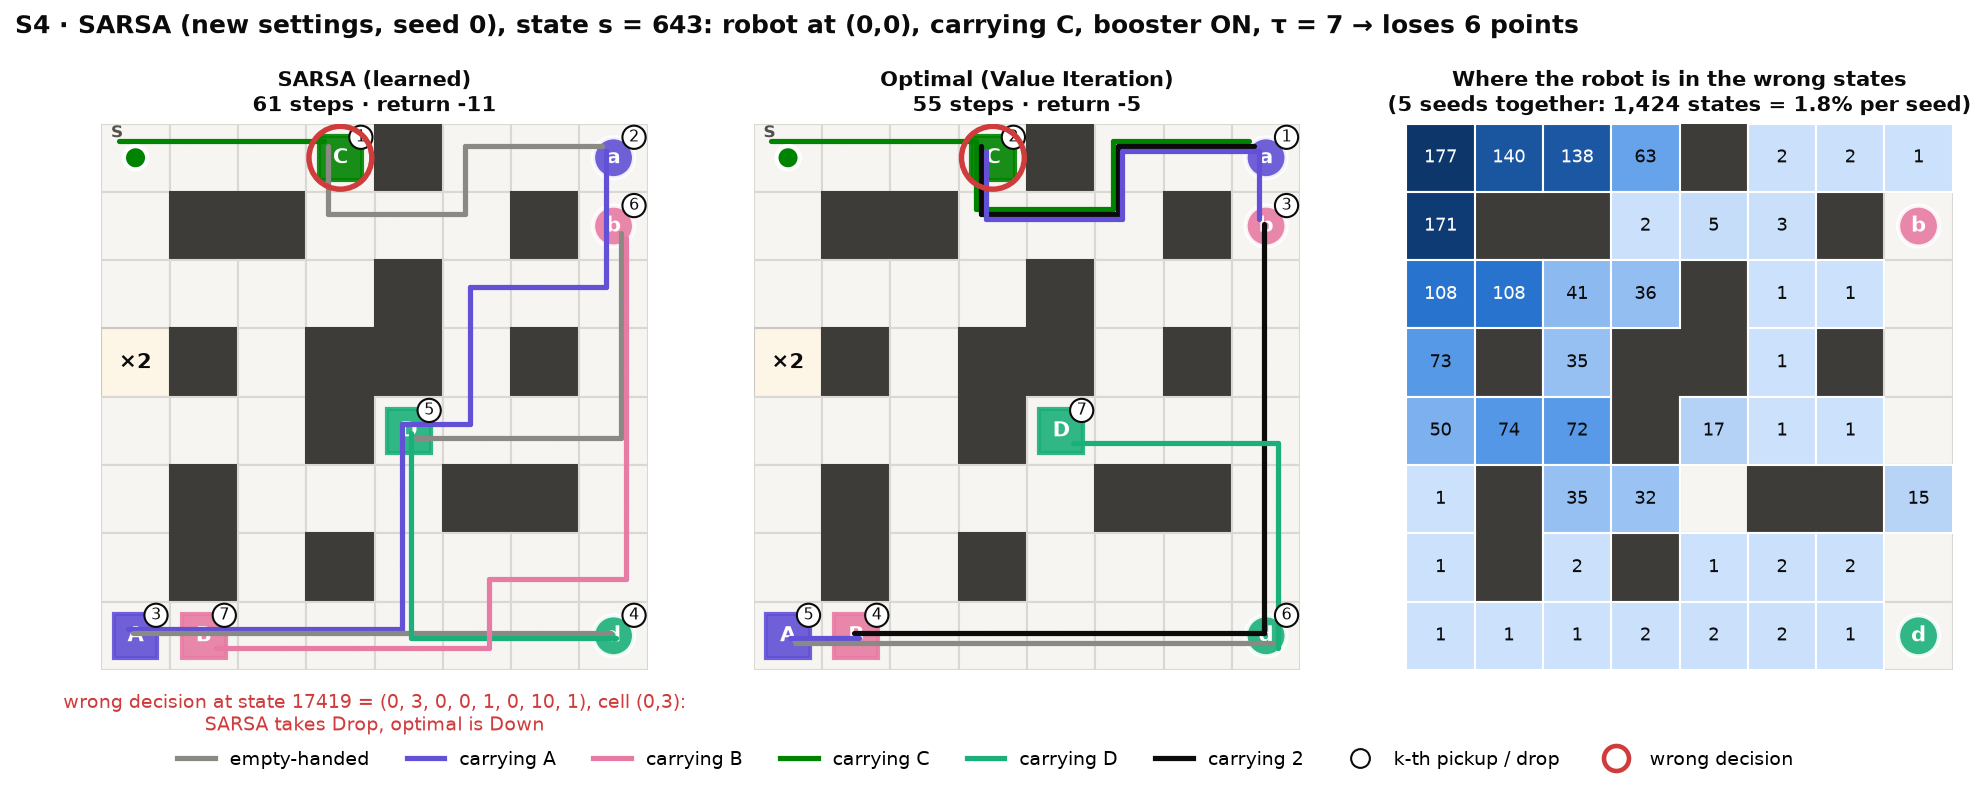
\includegraphics[width=\linewidth,height=0.62\textheight,keepaspectratio]{figures/fig11.png}
\caption{S4, SARSA: the costliest wrong state of seed 0, learned route (left) versus optimal route (middle), red ring = wrong decision; right: robot position in the wrong states of all 5 seeds}\label{fig:11}
\end{figure}

Where exactly does SARSA turn wrong? In the example the start state
(code 643) is fine: SARSA\textquotesingle s first action, Right, is
optimal. The wrong decision comes 3 steps later, at state code
\textbf{17419 = (0, 3, 0, 0, 1, 0, 10, 1)} on C\textquotesingle s drop
cell (red ring in Figure 11): SARSA drops C, while the optimal action is
Down. In Q* the two actions differ by only 0.04 (Down −9.89, Drop
−9.93): with γ = 0.99, delivering C at once brings its +20 forward,
which almost pays for the 6 extra steps it causes later.
SARSA\textquotesingle s Q values in this state are 0.12--0.24 below Q*,
more than that gap, so the order of the two actions flips.

All 301 wrong states of seed 0 come from only 39 wrong decisions (29--39
over the 5 seeds), and the ten most common ones cover 74\% of the wrong
states (Table 12). They sit on just two cells: (4, 2),
C\textquotesingle s pickup cell, where the robot carries B and C with
the booster on and SARSA goes Down instead of Up, and (0, 3),
C\textquotesingle s drop cell, where SARSA drops C instead of going
Down. In each of them Q* separates SARSA\textquotesingle s choice from
the optimal action by at most 0.04, so a small error in
SARSA\textquotesingle s Q table is enough to pick the wrong one.

\begin{longtable}[]{@{}
  >{\raggedright\arraybackslash}p{(\columnwidth - 12\tabcolsep) * \real{0.1045}}
  >{\raggedright\arraybackslash}p{(\columnwidth - 12\tabcolsep) * \real{0.2540}}
  >{\raggedright\arraybackslash}p{(\columnwidth - 12\tabcolsep) * \real{0.1045}}
  >{\raggedright\arraybackslash}p{(\columnwidth - 12\tabcolsep) * \real{0.1046}}
  >{\raggedright\arraybackslash}p{(\columnwidth - 12\tabcolsep) * \real{0.1084}}
  >{\raggedright\arraybackslash}p{(\columnwidth - 12\tabcolsep) * \real{0.1633}}
  >{\raggedright\arraybackslash}p{(\columnwidth - 12\tabcolsep) * \real{0.1607}}@{}}
\caption{S4, SARSA (seed 0): the ten most common wrong decisions, with their state code; values are given for SARSA\textquotesingle s action / the optimal action}\label{tab:12}\\
\toprule\noalign{}
\begin{minipage}[b]{\linewidth}\raggedright
\textbf{State code}
\end{minipage} & \begin{minipage}[b]{\linewidth}\raggedright
\textbf{State (row, col, σA, σB, σC, σD, τ, b)}
\end{minipage} & \begin{minipage}[b]{\linewidth}\raggedright
\textbf{Wrong states via it}
\end{minipage} & \begin{minipage}[b]{\linewidth}\raggedright
\textbf{SARSA takes}
\end{minipage} & \begin{minipage}[b]{\linewidth}\raggedright
\textbf{Optimal}
\end{minipage} & \begin{minipage}[b]{\linewidth}\raggedright
\textbf{True Q*}
\end{minipage} & \begin{minipage}[b]{\linewidth}\raggedright
\textbf{Learned Q}
\end{minipage} \\
\midrule\noalign{}
\endfirsthead
\caption[]{(continued)}\\
\toprule\noalign{}
\begin{minipage}[b]{\linewidth}\raggedright
\textbf{State code}
\end{minipage} & \begin{minipage}[b]{\linewidth}\raggedright
\textbf{State (row, col, σA, σB, σC, σD, τ, b)}
\end{minipage} & \begin{minipage}[b]{\linewidth}\raggedright
\textbf{Wrong states via it}
\end{minipage} & \begin{minipage}[b]{\linewidth}\raggedright
\textbf{SARSA takes}
\end{minipage} & \begin{minipage}[b]{\linewidth}\raggedright
\textbf{Optimal}
\end{minipage} & \begin{minipage}[b]{\linewidth}\raggedright
\textbf{True Q*}
\end{minipage} & \begin{minipage}[b]{\linewidth}\raggedright
\textbf{Learned Q}
\end{minipage} \\
\midrule\noalign{}
\endhead
\bottomrule\noalign{}
\endlastfoot
190921 & (4, 2, 0, 1, 1, 0, 22, 1) & 109 & Down & Up & 26.73 / 26.76 &
26.73 / 26.60 \\
190915 & (4, 2, 0, 1, 1, 0, 20, 1) & 20 & Down & Up & −2.97 / −2.94 &
−2.97 / −3.07 \\
190918 & (4, 2, 0, 1, 1, 0, 21, 1) & 20 & Down & Up & −3.27 / −3.24 &
−3.27 / −3.42 \\
190909 & (4, 2, 0, 1, 1, 0, 18, 1) & 17 & Down & Up & −2.38 / −2.35 &
−2.38 / −2.54 \\
190912 & (4, 2, 0, 1, 1, 0, 19, 1) & 17 & Down & Up & −2.68 / −2.64 &
−2.68 / −2.82 \\
17455 & (0, 3, 0, 0, 1, 0, 22, 1) & 15 & Drop & Down & 16.93 / 16.97 &
16.92 / 16.82 \\
190903 & (4, 2, 0, 1, 1, 0, 16, 1) & 7 & Down & Up & −1.80 / −1.77 &
−1.80 / −1.91 \\
190906 & (4, 2, 0, 1, 1, 0, 17, 1) & 7 & Down & Up & −2.09 / −2.06 &
−2.09 / −2.21 \\
17419 & (0, 3, 0, 0, 1, 0, 10, 1) & 5 & Drop & Down & −9.93 / −9.89 &
−10.05 / −10.13 \\
17422 & (0, 3, 0, 0, 1, 0, 11, 1) & 5 & Drop & Down & −10.21 / −10.17 &
−10.21 / −10.40 \\
\end{longtable}

Two variants test where the error comes from (Table 11). \textbf{Twice
as many episodes barely helps} (S4: 1.8\% → 1.8\% of the states), so the
mistakes are not caused by too short training. \textbf{A smaller final
step size helps}: with α decaying to 0.02 instead of 0.1, SARSA becomes
exact on S3 in all 5 seeds and the wrong states on S4 halve (0.9\%,
29--283 per seed). This fits the explanation in Section 8:
SARSA\textquotesingle s target r + γ·Q(s′, a′) is noisy because a′ is
sometimes random, a small α averages that noise out, and a gap of a few
hundredths between two actions in Q* is easily swapped by the error that
remains. Two quick tests on S4 (3 seeds each, outside failure\_cases.py)
point the same way: a constant α = 0.5 or α = 1 leaves 3,263--7,583
wrong states, and SARSA with Q-learning\textquotesingle s ε schedule (ε
→ 0.01) leaves 2,442--2,649, because on-policy SARSA then learns the
value of a policy that still explores.

\hypertarget{what-this-means}{%
\subsection{What this means}\label{what-this-means}}

\begin{itemize}
\item
  Accuracy from start cells is not the whole picture: a policy that is
  100\% correct from every start cell can still be wrong in states off
  its route. Checking every reachable state takes less than a second per
  Q table here and shows the difference.
\item
  For this task Q-learning and Monte Carlo ES are the safe choices:
  their Q tables are optimal in every state, so the robot finds the best
  route again even from an unusual state.
\item
  Every mistake can be traced to a state code. SARSA\textquotesingle s
  few hundred wrong states on S4 come from a few dozen wrong decisions
  on two cells, where two actions are almost equally good in Q*;
  Appendix A lists all of them with their state code, and
  results/failure\_states.csv lists every wrong state.
\item
  SARSA\textquotesingle s remaining mistakes are small (at most 6
  points, never a loop) and do not go away with more episodes; a smaller
  final step size removes about half of them on S4 and all of them on
  S3.
\end{itemize}

\hypertarget{conclusion-and-how-to-run-the-demo}{%
\section{Conclusion and how to run the
demo}\label{conclusion-and-how-to-run-the-demo}}

With 4 levelled maps, a state space of up to 357,696 encoded states
(15,612 reachable) and enough episodes, all three tabular algorithms
find the optimal delivery order by themselves, including prioritising
the deadline parcel and exploiting the booster cell.

\begin{itemize}
\item
  Q-learning, SARSA and Monte Carlo ES: 100\% accuracy in 5/5 seeds on
  all 4 maps (60/60 runs); the Q tables converge to Q*.
\item
  Exploring starts and a per-algorithm ε schedule are the key settings:
  they let every state be learned despite the deadline clock and the
  booster flag.
\item
  Q-learning learns the fastest and most stably; Monte Carlo ES is
  second; SARSA needs about 3 times as many episodes as Q-learning on S4
  and still fluctuates.
\item
  Started in every reachable state rather than only at a start cell,
  Q-learning and Monte Carlo ES are never wrong; SARSA takes a slightly
  longer route from 0.3\% of the S3 states and 1.8\% of the S4 states
  (at most 6 extra steps, never a loop) (Section 10).
\item
  The number of episodes matters on hard maps: S4 needs 1--4 million
  episodes depending on the algorithm; numba makes this run in a few
  tens of seconds.
\item
  Changing the reward (late penalty) or the environment (deadline,
  booster cell) changes the delivery order exactly as the optimal
  solution predicts.
\item
  The learned values make the task visible: they rise toward the current
  target, and cells from which the deadline can no longer be met become
  negative.
\end{itemize}

\textbf{Limitations.} The τ variable makes the state space grow linearly
with the deadline length. Exploring starts need a simulator that can put
the robot in any state, which is hard with a real robot. The Q table is
tied to one grid, so every map must be trained separately. The
hyperparameters were tuned on these same 4 maps. The accuracy of Section
6 only covers start cells; Section 10 shows that SARSA can still be
slightly wrong in states off its route.

\textbf{Future work.} Try a stochastic environment (wheel slip) to see
whether the ranking of the three algorithms changes; try Expected SARSA
or Q(λ), and a SARSA step-size schedule that is also exact off the
route; replace the Q table with function approximation so that one model
can serve several maps.

\textbf{Running everything again}

\begin{lstlisting}
pip install gymnasium numpy matplotlib numba
python experiments.py     # ~4 minutes on 12 CPU cores; --quick for a fast test
python plots.py --lang en # 17 figures with English labels in figures_en/
python convergence.py     # measures how Q converges to Q*
python failure_cases.py   # where each policy goes wrong (~3 min)
python demo.py            # one S4 episode with the learned policy, step by step
python demo.py --config configs/s3_deadline.json --algo sarsa --gif
python play.py            # play yourself: W/A/S/D move, J picks up, K drops
\end{lstlisting}

The demo prints a text map after every step (@ robot, a/b/c/d waiting
parcels, A/B/C/D drop cells, * delivered, + booster cell) with the
action, reward and event; on S4 it ends at step 67 with return 13.
play.py uses the same rules but lets you drive the robot with the
keyboard, and at the end compares your return with the optimal route. On
Google Colab, open colab\_train.ipynb and run the cells in order.

\hypertarget{appendix-a.-state-codes-of-every-wrong-decision}{%
\appendix
\section{State codes of every wrong
decision}\label{appendix-a.-state-codes-of-every-wrong-decision}}

Table 13 lists every different wrong decision of SARSA over the 5 seeds:
4 states on S3 and 56 on S4. State code = encode(s) (Section 3); the
state is written as (row, col, σ₁, \ldots, σ\textsubscript{N}, τ, b)
with σ = 0 waiting, 1 carried, 2 delivered. "Q* gap" is how much worse
SARSA\textquotesingle s action is than the optimal one in the true
values Q*. In 36 of the 60 wrong decisions the gap is at most 0.05, and
these cause 92\% of the wrong states: a small error in
SARSA\textquotesingle s Q table is enough to swap the two actions. The
other 24 have a gap of 0.24--1.24 (at most about one extra step) and
cause the remaining 8\%. Q-learning and Monte Carlo ES make no wrong
decision. Every wrong state, with its wrong decision, is in
results/failure\_states.csv.

\begin{longtable}[]{@{}
  >{\raggedright\arraybackslash}p{(\columnwidth - 14\tabcolsep) * \real{0.0706}}
  >{\raggedright\arraybackslash}p{(\columnwidth - 14\tabcolsep) * \real{0.1045}}
  >{\raggedright\arraybackslash}p{(\columnwidth - 14\tabcolsep) * \real{0.2443}}
  >{\raggedright\arraybackslash}p{(\columnwidth - 14\tabcolsep) * \real{0.1016}}
  >{\raggedright\arraybackslash}p{(\columnwidth - 14\tabcolsep) * \real{0.1102}}
  >{\raggedright\arraybackslash}p{(\columnwidth - 14\tabcolsep) * \real{0.0876}}
  >{\raggedright\arraybackslash}p{(\columnwidth - 14\tabcolsep) * \real{0.1258}}
  >{\raggedright\arraybackslash}p{(\columnwidth - 14\tabcolsep) * \real{0.1553}}@{}}
\caption{SARSA, 5 seeds: every wrong decision with its state code (sorted by map and by the number of wrong states that lead to it)}\label{tab:13}\\
\toprule\noalign{}
\begin{minipage}[b]{\linewidth}\raggedright
\textbf{Map}
\end{minipage} & \begin{minipage}[b]{\linewidth}\raggedright
\textbf{State code}
\end{minipage} & \begin{minipage}[b]{\linewidth}\raggedright
\textbf{State (row, col, σ\ldots, τ, b)}
\end{minipage} & \begin{minipage}[b]{\linewidth}\raggedright
\textbf{SARSA takes}
\end{minipage} & \begin{minipage}[b]{\linewidth}\raggedright
\textbf{Optimal}
\end{minipage} & \begin{minipage}[b]{\linewidth}\raggedright
\textbf{Q* gap}
\end{minipage} & \begin{minipage}[b]{\linewidth}\raggedright
\textbf{Seeds}
\end{minipage} & \begin{minipage}[b]{\linewidth}\raggedright
\textbf{Wrong states via it}
\end{minipage} \\
\midrule\noalign{}
\endfirsthead
\caption[]{(continued)}\\
\toprule\noalign{}
\begin{minipage}[b]{\linewidth}\raggedright
\textbf{Map}
\end{minipage} & \begin{minipage}[b]{\linewidth}\raggedright
\textbf{State code}
\end{minipage} & \begin{minipage}[b]{\linewidth}\raggedright
\textbf{State (row, col, σ\ldots, τ, b)}
\end{minipage} & \begin{minipage}[b]{\linewidth}\raggedright
\textbf{SARSA takes}
\end{minipage} & \begin{minipage}[b]{\linewidth}\raggedright
\textbf{Optimal}
\end{minipage} & \begin{minipage}[b]{\linewidth}\raggedright
\textbf{Q* gap}
\end{minipage} & \begin{minipage}[b]{\linewidth}\raggedright
\textbf{Seeds}
\end{minipage} & \begin{minipage}[b]{\linewidth}\raggedright
\textbf{Wrong states via it}
\end{minipage} \\
\midrule\noalign{}
\endhead
\bottomrule\noalign{}
\endlastfoot
S3 & 2408 & (0, 4, 0, 2, 0, 14, 0) & Down & Right & 1.07 & 3 & 46 \\
S3 & 27547 & (6, 6, 0, 2, 1, 16, 0) & Down & Left & 1.09 & 1 & 13 \\
S3 & 18153 & (4, 4, 0, 0, 0, 9, 0) & Up & Right & 0.25 & 0 & 2 \\
S3 & 19851 & (5, 0, 0, 0, 0, 6, 0) & Up & Down & 0.24 & 0 & 1 \\
S4 & 190921 & (4, 2, 0, 1, 1, 0, 22, 1) & Down & Up & 0.03 & all 5 &
543 \\
S4 & 190915 & (4, 2, 0, 1, 1, 0, 20, 1) & Down & Up & 0.03 & all 5 &
98 \\
S4 & 190918 & (4, 2, 0, 1, 1, 0, 21, 1) & Down & Up & 0.03 & all 5 &
98 \\
S4 & 190909 & (4, 2, 0, 1, 1, 0, 18, 1) & Down & Up & 0.03 & all 5 &
85 \\
S4 & 190912 & (4, 2, 0, 1, 1, 0, 19, 1) & Down & Up & 0.03 & all 5 &
83 \\
S4 & 17455 & (0, 3, 0, 0, 1, 0, 22, 1) & Drop & Down & 0.04 & all 5 &
71 \\
S4 & 190906 & (4, 2, 0, 1, 1, 0, 17, 1) & Down & Up & 0.03 & all 5 &
35 \\
S4 & 17425 & (0, 3, 0, 0, 1, 0, 12, 1) & Drop & Down & 0.04 & all 5 &
25 \\
S4 & 17431 & (0, 3, 0, 0, 1, 0, 14, 1) & Drop & Down & 0.04 & all 5 &
25 \\
S4 & 17452 & (0, 3, 0, 0, 1, 0, 21, 1) & Drop & Down & 0.04 & all 5 &
25 \\
S4 & 17437 & (0, 3, 0, 0, 1, 0, 16, 1) & Drop & Down & 0.04 & all 5 &
24 \\
S4 & 17440 & (0, 3, 0, 0, 1, 0, 17, 1) & Drop & Down & 0.04 & all 5 &
24 \\
S4 & 17443 & (0, 3, 0, 0, 1, 0, 18, 1) & Drop & Down & 0.04 & all 5 &
24 \\
S4 & 17446 & (0, 3, 0, 0, 1, 0, 19, 1) & Drop & Down & 0.04 & all 5 &
24 \\
S4 & 17449 & (0, 3, 0, 0, 1, 0, 20, 1) & Drop & Down & 0.04 & all 5 &
24 \\
S4 & 190903 & (4, 2, 0, 1, 1, 0, 16, 1) & Down & Up & 0.03 & 0, 1, 2 &
21 \\
S4 & 17422 & (0, 3, 0, 0, 1, 0, 11, 1) & Drop & Down & 0.04 & 0, 1, 3, 4
& 20 \\
S4 & 17428 & (0, 3, 0, 0, 1, 0, 13, 1) & Drop & Down & 0.04 & 0, 1, 3, 4
& 20 \\
S4 & 17434 & (0, 3, 0, 0, 1, 0, 15, 1) & Drop & Down & 0.04 & 0, 1, 3, 4
& 20 \\
S4 & 17419 & (0, 3, 0, 0, 1, 0, 10, 1) & Drop & Down & 0.04 & 0, 1, 3, 4
& 19 \\
S4 & 340962 & (7, 5, 0, 0, 0, 0, 11, 0) & Down & Right & 1.16 & 3 & 9 \\
S4 & 73958 & (1, 5, 0, 0, 2, 0, 19, 2) & Down & Up & 0.24 & 2 & 8 \\
S4 & 40418 & (0, 7, 0, 0, 2, 0, 17, 2) & Down & Pickup & 0.25 & 2 & 7 \\
S4 & 292545 & (6, 4, 0, 0, 0, 1, 18, 0) & Left & Up & 1.24 & 1 & 7 \\
S4 & 135025 & (3, 0, 0, 1, 1, 0, 20, 1) & Down & Up & 0.03 & all 5 &
5 \\
S4 & 135028 & (3, 0, 0, 1, 1, 0, 21, 1) & Down & Up & 0.03 & all 5 &
5 \\
S4 & 135031 & (3, 0, 0, 1, 1, 0, 22, 1) & Down & Up & 0.03 & all 5 &
5 \\
S4 & 202093 & (4, 4, 0, 1, 1, 0, 20, 1) & Down & Right & 0.03 & all 5 &
5 \\
S4 & 202096 & (4, 4, 0, 1, 1, 0, 21, 1) & Down & Right & 0.03 & all 5 &
5 \\
S4 & 202099 & (4, 4, 0, 1, 1, 0, 22, 1) & Down & Right & 0.03 & all 5 &
5 \\
S4 & 263572 & (5, 7, 0, 1, 1, 0, 20, 1) & Down & Up & 0.03 & all 5 &
5 \\
S4 & 263575 & (5, 7, 0, 1, 1, 0, 21, 1) & Down & Up & 0.03 & all 5 &
5 \\
S4 & 263578 & (5, 7, 0, 1, 1, 0, 22, 1) & Down & Up & 0.03 & all 5 &
5 \\
S4 & 135022 & (3, 0, 0, 1, 1, 0, 19, 1) & Down & Up & 0.03 & 0, 1, 2, 3
& 4 \\
S4 & 162732 & (3, 5, 0, 0, 1, 0, 10, 0) & Left & Up & 1.15 & 0 & 4 \\
S4 & 73314 & (1, 5, 0, 0, 1, 0, 12, 0) & Right & Left & 1.18 & 0 & 3 \\
S4 & 5647 & (0, 1, 0, 0, 0, 0, 19, 1) & Down & Right & 1.16 & 0 & 2 \\
S4 & 12467 & (0, 2, 0, 0, 2, 0, 15, 2) & Up & Right & 0.97 & 0 & 2 \\
S4 & 118023 & (2, 5, 0, 0, 1, 0, 11, 0) & Left & Up & 1.17 & 0 & 2 \\
S4 & 182227 & (4, 0, 0, 1, 2, 1, 22, 1) & Down & Right & 0.27 & 0 & 2 \\
S4 & 185320 & (4, 1, 0, 1, 1, 0, 18, 1) & Left & Right & 0.03 & 2, 3 &
2 \\
S4 & 185323 & (4, 1, 0, 1, 1, 0, 19, 1) & Left & Right & 0.03 & 2, 3 &
2 \\
S4 & 185326 & (4, 1, 0, 1, 1, 0, 20, 1) & Left & Right & 0.03 & 1, 2 &
2 \\
S4 & 195062 & (4, 2, 0, 0, 2, 2, 22, 2) & Down & Up & 0.55 & 0 & 2 \\
S4 & 298104 & (6, 5, 0, 0, 0, 1, 8, 0) & Up & Left & 1.23 & 1 & 2 \\
S4 & 5725 & (0, 1, 1, 0, 0, 0, 22, 1) & Left & Right & 0.25 & 3 & 1 \\
S4 & 67092 & (1, 4, 0, 0, 0, 0, 8, 0) & Right & Left & 0.93 & 2 & 1 \\
S4 & 67728 & (1, 4, 0, 0, 1, 0, 13, 0) & Up & Left & 1.19 & 0 & 1 \\
S4 & 68170 & (1, 4, 0, 2, 1, 0, 22, 1) & Left & Right & 0.26 & 2 & 1 \\
S4 & 178866 & (4, 0, 0, 0, 0, 0, 6, 0) & Right & Up & 0.58 & 2 & 1 \\
S4 & 185329 & (4, 1, 0, 1, 1, 0, 21, 1) & Left & Right & 0.03 & 3 & 1 \\
S4 & 185332 & (4, 1, 0, 1, 1, 0, 22, 1) & Left & Right & 0.03 & 1 & 1 \\
S4 & 203134 & (4, 4, 0, 0, 0, 1, 22, 1) & Drop & Down & 0.05 & 0 & 1 \\
S4 & 240360 & (5, 3, 0, 0, 0, 0, 11, 0) & Right & Left & 0.96 & 2 & 1 \\
S4 & 240591 & (5, 3, 0, 1, 0, 0, 19, 0) & Up & Left & 1.22 & 4 & 1 \\
S4 & 279483 & (6, 2, 0, 0, 0, 0, 11, 0) & Down & Up & 0.96 & 2 & 1 \\
\end{longtable}

\end{document}
